% Chinese gloss placed under an English paragraph (also defined in lec_4/lec_5; \lec groups each file).
\providecommand*{\zh}[1]{\par\smallskip{\small\color{MidnightBlue!80!black}\noindent【中】#1\par}\smallskip}

%─────Lecture 6──────────────────────────────────────────────────────────────────────────────────────────────────────────────────────────────────────
\chapter{Forwards, Futures, Futures Options, Swaps}
\label{ch:forwards}
\marginpar{\footnotesize\textsf{\raggedright Lecture 6\\ October 15, 2026}}

\source{Slides pp.~480--481}

\begin{flushright}
	\itshape Summon the nations to come to the trial.\\
	Which of their gods can predict the future?\\
	\upshape --- Isaiah 43:9
\end{flushright}

\begin{flushright}
	\itshape The sure fun of the evening\\
	outweighed the uncertain treasure[.]\\
	\upshape --- Mark Twain (1835--1910), \itshape The Adventures of Tom Sawyer
\end{flushright}

\bigskip

\source{Slides pp.~482--483}

\begin{notation}
	\begin{itemize}[nosep]
		\item $r$: the riskless interest rate; continuous compounding is assumed.
		\item $t$: the current time; $T$: the maturity date; $\tau\triangleq T-t$: the remaining time to maturity (years).
		\item $S$: the spot price; $S_{T}$: the spot price at maturity.
		\item $X$: the delivery price.
		\item $F$: the forward or futures price for a newly written contract.
		\item $f$: the value of the contract.
		\item A price with a subscript $t$ usually refers to the price at time $t$.
	\end{itemize}
\end{notation}

\zh{$r$ 是無風險利率（連續複利），$t$ 是現在、$T$ 是到期日、$\tau=T-t$ 是剩餘期間；$S$ 是現貨價、$S_{T}$ 是到期時的現貨價；$X$ 是交割價（delivery price）；$F$ 是新簽合約的 forward/futures price；$f$ 是合約的價值；下標 $t$ 通常代表時間 $t$ 的價格。}

\begin{remark}
	$X$ 和 $F$ 要分清楚：$X$ 是\emph{寫在合約上}、簽約後不變的交割價；$F$ 是\emph{現在}新簽一份合約會用的交割價，隨市場變動。合約剛簽時 $X=F$。
\end{remark}

%─────§ Forward contracts────────────────────────────────────────────────────────────────────────────────────────────────────────────────────────────
\section{Forward Contracts}
\label{sec:forward-contracts}

\source{Slides pp.~484--485}

Long \vocab{forward contracts} are for the purchase of the underlying asset for a certain delivery price on a specific time.\footnote{They have a 4,000-year history (Marthinsen, 2018).}
The underlying can be foreign currencies, bonds, corn, etc.
They are ideal for hedging purposes.
For example, a farmer enters into a forward contract with a food processor to deliver 100,000 bushels of corn for \$2.5 per bushel on September 27, 1995.\footnote{The farmer assumes a short position.}
The farmer is assured of a buyer at an acceptable price, and the processor knows the cost of corn in advance.

\zh{long forward contract 是約定在特定時間、以特定交割價買入標的資產的合約，標的可以是外幣、債券、玉米等，很適合避險。例：農夫和食品加工廠簽約，1995/9/27 以每 bushel 2.5 元交 10 萬 bushels 玉米（農夫是 short 方）。農夫確保有買家、價格可接受；加工廠事先知道成本。}

A forward agreement limits both risk and rewards.
If the spot price of corn rises on the delivery date, the farmer will miss the opportunity of extra profits; if the price declines, the processor will be paying more than it would.
Either side has an incentive to default.
Other problems: the food processor may go bankrupt, the farmer can go bust, the farmer might not be able to harvest 100,000 bushels of corn because of bad weather, the cost of growing corn may skyrocket, etc.

\zh{forward 同時限制了風險和報酬：交割日玉米漲價，農夫少賺；跌價，加工廠多付。所以雙方都有違約的誘因。其他問題：加工廠可能倒閉、農夫可能破產、天候不佳收成不到 10 萬 bushels、種植成本暴漲等。}

\subsection{Spot and Forward Exchange Rates}
\label{sec:irp}

\source{Slides pp.~486--488}

\begin{notation}
	\begin{itemize}[nosep]
		\item $S$: the spot exchange rate; $F$: the forward exchange rate one year from now (both in domestic/foreign terms, as in \autoref{sec:forex});
		\item $r_{f}$: the annual interest rate of the foreign currency; $r$: the annual interest rate of the local currency.
	\end{itemize}
\end{notation}

Arbitrage opportunities will arise unless these four numbers satisfy an equation, due to Keynes (1923).\footnote{John Maynard Keynes (1883--1946) was one of the greatest economists in history. The parity broke down in late 2008 (Mancini-Griffoli \& Ranaldo, 2013).}

\begin{theorem}[Interest rate parity]
	\label{thm:irp}
	\begin{equation}
		\frac{F}{S} \;=\; e^{r-r_{f}} .
		\label{eq:irp}
	\end{equation}
\end{theorem}

\begin{proof}
	A holder of the local currency can do either of:
	\begin{enumerate}[(1),nosep]
		\item lend the money in the domestic market to receive $e^{r}$ one year from now;
		\item convert local currency for foreign currency, lend for 1 year in the foreign market, and convert foreign currency into local currency at the fixed forward exchange rate $F$, by selling forward foreign currency now.
	\end{enumerate}
	No money changes hand in entering into a forward contract, so one unit of local currency becomes $Fe^{r_{f}}/S$ one year from now in the second case.
	If $Fe^{r_{f}}/S>e^{r}$, an arbitrage profit can result from borrowing money in the domestic market and lending it in the foreign market.
	If $Fe^{r_{f}}/S<e^{r}$, an arbitrage profit can result from borrowing money in the foreign market and lending it in the domestic market.
\end{proof}

\zh{記 $S$ 為即期匯率、$F$ 為一年期遠期匯率（都是「本國貨幣/外幣」），$r_{f}$、$r$ 分別是外國、本國年利率。四個數必須滿足 interest rate parity \eqref{eq:irp}，否則有套利。證明：一單位本國貨幣可以 (1) 存在本國，一年後得 $e^{r}$；(2) 換成外幣（$1/S$）、存在外國（變成 $e^{r_{f}}/S$）、並用 forward 鎖定以 $F$ 換回，一年後得 $Fe^{r_{f}}/S$。簽 forward 不用付錢，所以兩者必須相等；較大的那邊借另一邊的錢來投資就是套利。}

\begin{remark}
	\textbf{(2) 的 $Fe^{r_{f}}/S$ 怎麼來。}$1$ 單位本國貨幣換成 $1/S$ 單位外幣；在外國存一年變成 $e^{r_{f}}/S$ 單位外幣；今天先賣出這麼多外幣的 forward，一年後每單位外幣換回 $F$ 單位本國貨幣，共 $Fe^{r_{f}}/S$。整個過程只有今天的 $1$ 和一年後的 $Fe^{r_{f}}/S$ 兩筆現金流，沒有任何風險，所以必須和 (1) 的 $e^{r}$ 相等。
	\eqref{eq:irp} 也是下面 \eqref{eq:fwd-price-q} 取 $q=r_{f}$、$\tau=1$ 的特例：外幣就是 dividend yield 為 $r_{f}$ 的資產（\autoref{sec:forex}）。
\end{remark}

\subsection{Forward Price}

\source{Slides pp.~489--491}

The payoff of a forward contract at maturity is
\[
	S_{T}-X .
\]
Contrast that with the call's payoff $\max(S_{T}-X,0)$ \eqref{eq:call-payoff}.
Forward contracts do not involve any initial cash flow (\autoref{fig:forward-cashflow}).

\begin{definition}
	The \vocab{forward price} $F$ is the delivery price $X$ which makes the forward contract zero valued; that is, $f=0$ when $X=F$.
\end{definition}

\begin{figure}[H]
	\centering
	\begin{tikzpicture}[font=\small, >={Stealth[length=5pt]}]
		\draw[->] (0,0) -- (8.2,0);
		\foreach \x/\l in {0/0, 1.5/1, 3/2, 4.5/3, 7.5/n} \draw (\x,0.08) -- (\x,-0.08) node[below] {$\l$};
		\node[below] at (6,-0.08) {$\cdots$};
		\draw[->, thick, MidnightBlue!80!black] (7.5,0.15) -- (7.5,1.3) node[above] {$S_{T}-X$};
	\end{tikzpicture}
	\caption{Cash flow of a long forward contract: nothing at time $0$, a single
		cash flow $S_{T}-X$ (of either sign) at maturity.}
	\label{fig:forward-cashflow}
\end{figure}

The delivery price cannot change because it is written in the contract.
But the forward price may change after the contract comes into existence.
So although the value of a forward contract, $f$, is $0$ at the outset, it will fluctuate thereafter: this value is enhanced when the spot price climbs and depressed when the spot price declines.
The forward price also varies with the maturity of the contract.

\zh{forward 到期的 payoff 是 $S_{T}-X$（對比 call 的 $\max(S_{T}-X,0)$），期初沒有現金流。forward price $F$ 定義為讓合約價值 $f=0$ 的交割價。交割價寫在合約上不會變，但 forward price 會變，所以合約價值一開始是 $0$，之後會隨現貨價漲而漲、跌而跌；forward price 也隨合約期限而不同。}

\subsection{Underlying Pays No Income}

\source{Slides pp.~492--493}

\begin{lemma}
	\label{lem:fwd-no-income}
	For a forward contract on an underlying asset providing no income,
	\begin{equation}
		F \;=\; Se^{r\tau} .
		\label{eq:fwd-price}
	\end{equation}
\end{lemma}

\begin{proof}
	If $F>Se^{r\tau}$:
	borrow $S$ dollars for $\tau$ years, buy the underlying asset, and short the forward contract with delivery price $F$.
	At maturity, deliver the asset for $F$ and use $Se^{r\tau}$ to repay the loan, leaving an arbitrage profit of $F-Se^{r\tau}>0$.
	If $F<Se^{r\tau}$, do the opposite.
\end{proof}

\zh{標的不配息時，forward price 是 $F=Se^{r\tau}$ \eqref{eq:fwd-price}。若 $F>Se^{r\tau}$：借 $S$ 買資產、同時 short forward，到期以 $F$ 交出資產、還 $Se^{r\tau}$，淨賺 $F-Se^{r\tau}>0$。反之則反向操作（放空資產、把錢存起來、long forward）。}

\begin{remark}
	\textbf{「do the opposite」具體是什麼。}若 $F<Se^{r\tau}$：今天放空資產得 $S$、存起來，並 long forward（交割價 $F$）。到期存款變成 $Se^{r\tau}$，付 $F$ 收到資產、還給借券的人，淨賺 $Se^{r\tau}-F>0$。兩個方向都是今天零成本、到期確定正報酬，違反 \autoref{cor:zero-pv}。
\end{remark}

\source{Slides pp.~494--495}

\begin{eg}[Zero-coupon bonds]
	Let $r$ be the annualized 3-month riskless interest rate and $S$ the spot price of the 6-month zero-coupon bond.
	A new 3-month forward contract on that 6-month zero-coupon bond should command a delivery price of $Se^{r/4}$.
	So if $r=6\%$ and $S=970.87$, then the delivery price is
	\[
		970.87\times e^{0.06/4} \;=\; 985.54 .
	\]
\end{eg}

\begin{eg}[Options]
	Suppose $S$ is the spot price of the European call that expires at some time later than $T$.
	A $\tau$-year forward contract on that call commands a delivery price of $Se^{r\tau}$.
	So it equals the future value of the Black--Scholes formula (\autoref{thm:black-scholes}).
\end{eg}

\zh{例：$r$ 為 3 個月期年化利率、$S$ 為 6 個月期 zero-coupon bond 的現價，3 個月期的 forward 交割價是 $Se^{r/4}$；$r=6\%$、$S=970.87$ 時是 $985.54$。例：標的是比 $T$ 晚到期的 European call，$\tau$ 年期 forward 的交割價是 $Se^{r\tau}$，也就是 Black--Scholes 價格的終值。}

\begin{remark}
	兩個例子都直接套 \eqref{eq:fwd-price}，因為 zero-coupon bond 和 call 在 forward 期間都不發任何現金。第一個例子 $\tau=3/12=1/4$，所以 $e^{r\tau}=e^{0.06/4}$。
\end{remark}

\source{Slides pp.~496--498}

\begin{proposition}
	\label{prop:fwd-value}
	The value of a forward contract on an underlying asset paying no income is
	\begin{equation}
		f \;=\; S-Xe^{-r\tau} .
		\label{eq:fwd-value}
	\end{equation}
\end{proposition}

\begin{proof}
	Consider a portfolio consisting of one long forward contract, cash amount $Xe^{-r\tau}$, and one short position in the underlying asset.
	The cash will grow to $X$ at maturity, which can be used to take delivery of the forward contract.
	The delivered asset will then close out the short position.
	Since the value of the portfolio is zero at maturity, its PV must be zero (\autoref{cor:zero-pv}): $f+Xe^{-r\tau}-S=0$.
\end{proof}

So a forward contract can be replicated by a long position in the underlying and a loan of $Xe^{-r\tau}$ dollars.
\autoref{lem:fwd-no-income} is recovered by setting $f=0$ in \eqref{eq:fwd-value}: then $X=Se^{r\tau}$, the forward price.

\zh{不配息時 forward 合約的價值是 $f=S-Xe^{-r\tau}$ \eqref{eq:fwd-value}：持有 long forward、現金 $Xe^{-r\tau}$、放空一單位資產，到期現金變 $X$ 用來交割、拿到的資產拿去回補空頭，組合到期價值為 $0$，所以現值為 $0$。因此 forward $=$ 買資產 $+$ 借 $Xe^{-r\tau}$。在 \eqref{eq:fwd-value} 令 $f=0$ 就得到 $X=Se^{r\tau}$，即 \autoref{lem:fwd-no-income}。}

\begin{note}
	和 put--call parity \eqref{eq:put-call-parity} 比較：$C-P=S-\mathrm{PV}(X)$，右邊正是 \eqref{eq:fwd-value}。因為 long call $+$ short put 到期付 $\max(S_{T}-X,0)-\max(X-S_{T},0)=S_{T}-X$，就是一個交割價 $X$ 的 forward。
\end{note}

\subsection{Underlying Pays Predictable Income}

\source{Slides pp.~499--501}

\begin{lemma}
	\label{lem:fwd-income}
	For a forward contract on an underlying asset providing a predictable income with a PV of $I$,
	\begin{equation}
		F \;=\; (S-I)\,e^{r\tau} .
		\label{eq:fwd-price-income}
	\end{equation}
\end{lemma}

\begin{proof}
	If $F>(S-I)\,e^{r\tau}$, borrow $S$ dollars for $\tau$ years, buy the underlying asset, and short the forward contract with delivery price $F$.
	Use the income to repay part of the loan.
	At maturity, the asset is delivered for $F$, and $(S-I)\,e^{r\tau}$ is used to repay the remaining loan.
	That leaves an arbitrage profit of $F-(S-I)\,e^{r\tau}>0$.
	If $F<(S-I)\,e^{r\tau}$, reverse the above.
\end{proof}

\zh{標的有可預期收入、現值為 $I$ 時，$F=(S-I)e^{r\tau}$。若 $F$ 較大：借 $S$ 買資產、short forward，收到的收入拿去還一部分借款；到期交出資產拿 $F$，剩下的借款是 $(S-I)e^{r\tau}$，淨賺 $F-(S-I)e^{r\tau}>0$。}

\begin{remark}
	\textbf{為什麼剩下的借款是 $(S-I)e^{r\tau}$。}把借的 $S$ 拆成兩筆：$I$ 和 $S-I$。收入在各時點收到，現值合計 $I$，所以這些收入剛好還清第一筆 $I$ 的本息；第二筆 $S-I$ 到期本息為 $(S-I)e^{r\tau}$。
\end{remark}

\begin{eg}
	Consider a 10-month forward contract on a \$50 stock.
	The stock pays a dividend of \$1 every 3 months.
	The forward price is
	\[
		\bigl(50-e^{-r_{3}/4}-e^{-r_{6}/2}-e^{-3\times r_{9}/4}\bigr)\,e^{r_{10}\times(10/12)} ,
	\]
	where $r_{i}$ is the annualized $i$-month interest rate.
\end{eg}

\zh{例：股價 50、每 3 個月配息 1 元，10 個月期 forward price 如上，$r_{i}$ 是 $i$ 個月期的年化利率。}

\begin{remark}
	10 個月內配息發生在第 $3,6,9$ 個月，各 \$1，所以 $I=e^{-r_{3}\cdot3/12}+e^{-r_{6}\cdot6/12}+e^{-r_{9}\cdot9/12}$；每筆用自己期限的利率折現。再代入 \eqref{eq:fwd-price-income}，$\tau=10/12$。
\end{remark}

\subsection{Underlying Pays a Continuous Dividend Yield}
\label{sec:fwd-yield}

\source{Slide p.~502}

\begin{proposition}
	\label{prop:fwd-yield}
	If the underlying asset pays a continuous dividend yield of $q$, the value of a forward contract at any time prior to $T$ is
	\begin{equation}
		f \;=\; Se^{-q\tau}-Xe^{-r\tau} .
		\label{eq:fwd-value-q}
	\end{equation}
	Consequently the forward price is
	\begin{equation}
		F \;=\; Se^{(r-q)\tau} .
		\label{eq:fwd-price-q}
	\end{equation}
\end{proposition}

\begin{proof}[Proof（補充；簡報指向課本 p.~160）]
	買 $e^{-q\tau}$ 單位資產（成本 $Se^{-q\tau}$），收到的股利全部再買資產，則持有量以速率 $q$ 成長，到期剛好是 $e^{-q\tau}e^{q\tau}=1$ 單位，價值 $S_{T}$；再借 $Xe^{-r\tau}$，到期還 $X$。這個組合到期付 $S_{T}-X$，和 forward 相同，由 \autoref{cor:same-payoff}，$f=Se^{-q\tau}-Xe^{-r\tau}$。令 $f=0$ 解 $X$ 得 \eqref{eq:fwd-price-q}。
\end{proof}

\zh{標的有連續 dividend yield $q$ 時，合約價值 $f=Se^{-q\tau}-Xe^{-r\tau}$ \eqref{eq:fwd-value-q}，forward price $F=Se^{(r-q)\tau}$ \eqref{eq:fwd-price-q}。}

%─────§ Futures──────────────────────────────────────────────────────────────────────────────────────────────────────────────────────────────────────
\section{Futures Contracts}
\label{sec:futures}

\source{Slides pp.~503--504}

\vocab{Futures contracts} differ from forward contracts in the following ways:
\begin{itemize}[nosep]
	\item They are traded on a central exchange.
	\item There is a clearinghouse, so credit risk is minimized.
	\item Futures contracts are standardized instruments.
	\item Gains and losses are \vocab{marked to market} daily: adjusted at the end of each trading day based on the settlement price.
\end{itemize}

\zh{futures 和 forward 的差別：在集中交易所交易；有結算所（clearinghouse），信用風險降到最低；是標準化商品；每天 marked to market，依結算價在每個交易日結束時調整損益。}

The \vocab{size} of a futures contract is the amount of the underlying asset to be delivered under the contract: 5,000 bushels for the corn futures on the Chicago Board of Trade (CBOT); one million U.S.\ dollars for the Eurodollar futures on the Chicago Mercantile Exchange (CME).\footnote{CME and CBOT merged on July 12, 2007.}
A position can be closed out (or offset) by entering into a reversing trade to the original one.
Most futures contracts are closed out in this way rather than have the underlying asset delivered.
Forward contracts, by contrast, are meant for delivery.

\zh{futures 的合約規模是一口要交割的標的數量，例如 CBOT 玉米期貨 5{,}000 bushels、CME 歐洲美元期貨一百萬美元。部位可以用反向交易平倉（offset），大部分 futures 都是這樣了結而不實際交割；forward 則是為了交割。}

\subsection{Daily Settlements}

\source{Slides pp.~505--506}

Price changes in the futures contract are settled daily.
Hence the spot price rather than the initial futures price is paid on the delivery date.
Marking to market nullifies any financial incentive for not making delivery.

\begin{eg}
	A farmer enters into a forward contract to sell 100,000 bushels of corn at \$2.00 per bushel in November.
	Suppose the price of corn rises to \$2.5 by November.
	The farmer has incentive to sell his harvest in the spot market for \$2.5.
	With marking to market, the farmer has transferred \$0.5 per bushel from his futures account to that of the clearinghouse by November (\autoref{fig:daily-cashflow}).
	When the farmer makes delivery, he is paid the spot price, \$2.5 per bushel.
	The farmer has little incentive to default.
	The net price remains $\$2.5-0.5=2$ per bushel, the original delivery price.
\end{eg}

\zh{futures 每天結算價差，所以交割日付的是當時的現貨價而不是原本的 futures price。marking to market 消除了不交割的財務誘因。例：農夫約定 11 月以每 bushel 2 元賣玉米，11 月漲到 2.5 元，用 forward 的話農夫有誘因違約去現貨市場賣 2.5。用 futures 時，到 11 月農夫的保證金帳戶已經陸續付給結算所每 bushel 0.5；交割時拿到現貨價 2.5，淨價仍是 $2.5-0.5=2$，等於原本的交割價，違約沒有好處。}

\subsection{Daily Cash Flows}

\source{Slides pp.~507--508}

Let $F_{i}$ denote the futures price at the end of day $i$.
The contract's cash flow on day $i$ is $F_{i}-F_{i-1}$.
The net cash flow over the life of the contract is
\begin{equation}
	(F_{1}-F_{0})+(F_{2}-F_{1})+\cdots+(F_{n}-F_{n-1}) \;=\; F_{n}-F_{0} \;=\; S_{T}-F_{0} .
	\label{eq:futures-cashflow}
\end{equation}
A futures contract has the same accumulated payoff $S_{T}-F_{0}$ as a forward contract.
The actual payoff may vary because of the reinvestment of daily cash flows and how $S_{T}-F_{0}$ is distributed.

\begin{figure}[H]
	\centering
	\begin{tikzpicture}[font=\small, >={Stealth[length=5pt]}]
		\draw[->] (0,0) -- (8.2,0);
		\foreach \x/\l in {0/0, 1.5/1, 3/2, 4.5/3, 7.5/n} \draw (\x,0.08) -- (\x,-0.08) node[below] {$\l$};
		\node[below] at (6,-0.08) {$\cdots$};
		\draw[->, thick, MidnightBlue!80!black] (1.5,0.15) -- (1.5,1.0) node[above] {$F_{1}-F_{0}$};
		\draw[->, thick, RawSienna] (3,-0.45) -- (3,-1.2) node[below] {$F_{2}-F_{1}$};
		\draw[->, thick, RawSienna] (4.5,-0.45) -- (4.5,-1.0) node[below] {$F_{3}-F_{2}$};
		\draw[->, thick, MidnightBlue!80!black] (7.5,0.15) -- (7.5,1.2) node[above] {$F_{n}-F_{n-1}$};
	\end{tikzpicture}
	\caption{Daily cash flows of a long futures position: one cash flow per day, up
		or down, summing to $S_{T}-F_{0}$ by \eqref{eq:futures-cashflow}. Compare the
		single cash flow of \autoref{fig:forward-cashflow}.}
	\label{fig:daily-cashflow}
\end{figure}

\zh{令 $F_{i}$ 為第 $i$ 天收盤的 futures price，第 $i$ 天的現金流是 $F_{i}-F_{i-1}$，全部加起來 telescoping 成 $F_{n}-F_{0}=S_{T}-F_{0}$ \eqref{eq:futures-cashflow}，和 forward 的累積 payoff 一樣。實際 payoff 會因每天現金流的再投資、以及 $S_{T}-F_{0}$ 怎麼分配在各天而不同。}

\begin{remark}
	\eqref{eq:futures-cashflow} 最後一步 $F_{n}=S_{T}$：第 $n$ 天是交割日，交割日的結算價由現貨價決定（下一小節），所以 $F_{n}=S_{T}$。
\end{remark}

\subsection{Delivery and Hedging}

\source{Slide p.~509}

Futures price is the delivery price that makes the futures contract zero-valued.
Delivery ties the futures price to the spot price: on the delivery date, the settlement price of the futures contract is determined by the spot price.
Hence, when the delivery period is reached, the futures price should be very close to the spot price.\footnote{But since early 2006, futures for corn, wheat, and soybeans occasionally expired at a price much higher than that day's spot price (Henriques, 2008).}
Changes in futures prices usually track those in spot price, making hedging possible.

\zh{futures price 是讓 futures 合約價值為 $0$ 的交割價。交割把 futures price 和現貨價綁在一起：交割日的結算價由現貨價決定，所以接近交割期時 futures price 應該很接近現貨價。futures price 的變動通常跟著現貨價走，因此可以用來避險。}

\subsection{Forward and Futures Prices}

\source{Slides pp.~510--511}

Surprisingly, futures price equals forward price if interest rates are nonstochastic!\footnote{Cox, Ingersoll, \& Ross (1981); see p.~164 of the textbook for proof.}
This result ``justifies'' treating a futures contract as if it were a forward contract, ignoring its marking-to-market feature.
The West Texas Intermediate (WTI) futures price was negative on April 20, 2020!\footnote{April 21 was the last trading day for oil delivery in May to Cushing, Oklahoma.}

\zh{驚人的是，只要利率不是隨機的，futures price 就等於 forward price。這「合理化」了把 futures 當成 forward、忽略 marking to market 的做法。WTI 原油期貨在 2020/4/20 曾經是負價格。}

\begin{proposition}[Cox, Ingersoll, \& Ross, 1981]
	\label{prop:fwd-eq-futures}
	If the daily interest rate is a known constant $\delta$, then $F_{0}=G$, where $F_{0}$ is the futures price and $G$ the forward price, both for delivery on day $n$.
\end{proposition}

\begin{proof}[Proof（補充）]
	比較兩個策略在第 $n$ 天的價值。
	\begin{enumerate}[(1),nosep]
		\item \textbf{futures 策略。}今天存 $F_{0}$ 元；在第 $i$ 天開始時持有 $e^{i\delta}$ 口 long futures（$\delta$ 已知，所以口數事先決定）。第 $i$ 天的損益 $(F_{i}-F_{i-1})e^{i\delta}$ 以利率 $\delta$ 存到第 $n$ 天，變成 $(F_{i}-F_{i-1})e^{n\delta}$。由 \eqref{eq:futures-cashflow}，合計 $(S_{T}-F_{0})e^{n\delta}$，加上存款 $F_{0}e^{n\delta}$，總共 $S_{T}e^{n\delta}$。期初成本 $F_{0}$（futures 本身不用錢）。
		\item \textbf{forward 策略。}今天存 $G$ 元、long $e^{n\delta}$ 口交割價 $G$ 的 forward。第 $n$ 天得 $(S_{T}-G)e^{n\delta}+Ge^{n\delta}=S_{T}e^{n\delta}$。期初成本 $G$。
	\end{enumerate}
	兩個策略在每個 state 的 payoff 都是 $S_{T}e^{n\delta}$，由 \autoref{cor:same-payoff}，$F_{0}=G$。
\end{proof}

When interest rates are stochastic, forward and futures prices are no longer theoretically identical.
Suppose interest rates are uncertain and futures prices move in the same direction as interest rates.
Then futures prices will exceed forward prices.
For short-term contracts, the differences tend to be small.
Unless stated otherwise, assume forward and futures prices are identical.

\zh{利率是隨機時兩者理論上不再相等。若 futures price 和利率同方向變動，futures price 會高於 forward price。短期合約差異通常很小。除非特別說明，以下假設兩者相等。}

\begin{intuition}
	\autoref{prop:fwd-eq-futures} 的證明在 (1) 需要事先知道口數 $e^{i\delta}$，也就是利率必須是確定的。若 futures price 和利率正相關，long futures 賺錢時利率也高、賺的錢以高利率再投資，賠錢時利率低、借錢的成本也低，所以 long futures 比 long forward 有利；要讓兩者期初價值都是 $0$，futures 的交割價就必須更高。
\end{intuition}

%─────§ Futures options──────────────────────────────────────────────────────────────────────────────────────────────────────────────────────────────
\section{Futures Options and Forward Options}
\label{sec:futures-options}

\source{Slides pp.~512--513}

The underlying of a \vocab{futures option} is a futures contract.
Upon exercise, the option holder takes a position in the futures contract with a futures price equal to the option's strike price:
a call holder acquires a long futures position, and a put holder acquires a short futures position.
The futures contract is then marked to market, and the futures positions of the two parties are at the prevailing futures price (thus zero-valued).

It works as if the call holder received a futures contract plus cash equivalent to the prevailing futures price $F_{t}$ minus the strike price $X$, i.e., $F_{t}-X$; this futures contract has zero value.
It works as if the put holder sold a futures contract for $X-F_{t}$ dollars.

\zh{futures option 的標的是 futures 合約。履約時持有人取得一個 futures price 等於 strike 的 futures 部位：call 拿到 long、put 拿到 short。接著馬上 marked to market，雙方部位變成以當時的 futures price 計價（價值為 $0$）。所以效果等於 call 持有人拿到一份價值 $0$ 的 futures 加上現金 $F_{t}-X$；put 持有人則是拿到 $X-F_{t}$。}

\source{Slides pp.~514--515}

For a \vocab{forward option}, what is delivered is now a forward contract with a delivery price equal to the option's strike price.
Exercising a call forward option results in a long position in a forward contract; exercising a put forward option results in a short position in a forward contract.
Exercising a forward option incurs no immediate cash flows as there is no marking to market.

\zh{forward option 履約後拿到的是交割價等於 strike 的 forward 合約：call 拿到 long、put 拿到 short。因為沒有 marking to market，履約當下沒有現金流。}

\begin{eg}
	Consider an American call with strike \$100 and an expiration date in September.
	The underlying asset is a forward contract with a delivery date in December.
	Suppose the forward price in July is \$110.
	Upon exercise, the call holder receives a forward contract with a delivery price of \$100.
	If an offsetting position is then taken in the forward market,\footnote{The counterparty will pay you \$110 for the underlying asset.} a \$10 profit in December will be assured.
	A call on the futures would realize the \$10 profit in July.
\end{eg}

\zh{例：strike 100、9 月到期的 American call，標的是 12 月交割的 forward。7 月時 forward price 為 110，履約得到交割價 100 的 forward；再 short 一個交割價 110 的 forward 對沖，12 月確定賺 10。若是以 futures 為標的的 call，7 月就實現這 10 元。}

\subsection{Some Pricing Relations}

\source{Slides pp.~516--517}

Let $T$ be the delivery date, the current time be $0$, and the option (on the futures or forward contract) have expiration date $t$ ($t\le T$).
Assume a constant, positive interest rate.
Although forward price equals futures price, a forward option does not have the same value as a futures option.
The payoffs of calls at time $t$ are, respectively,
\begin{align}
	\text{futures option} & \;=\; \max(F_{t}-X,0) , \label{eq:futures-option-payoff} \\
	\text{forward option} & \;=\; \max(F_{t}-X,0)\,e^{-r(T-t)} . \label{eq:forward-option-payoff}
\end{align}

\zh{令 $T$ 為交割日、現在為 $0$、option 在 $t\le T$ 到期，利率為正的常數。雖然 forward price 等於 futures price，forward option 和 futures option 的價值卻不同：在時間 $t$ 的 payoff 分別是 \eqref{eq:futures-option-payoff} 和 \eqref{eq:forward-option-payoff}。}

\begin{remark}
	\textbf{\eqref{eq:forward-option-payoff} 的 $e^{-r(T-t)}$。}在 $t$ 履約 forward call 拿到交割價 $X$ 的 long forward，此時新的 forward price 是 $F_{t}$。由 \eqref{eq:fwd-value} 加上 \eqref{eq:fwd-price}（$S_{t}=F_{t}e^{-r(T-t)}$），它在 $t$ 的價值是
	\[
		S_{t}-Xe^{-r(T-t)} \;=\; (F_{t}-X)\,e^{-r(T-t)} :
	\]
	同樣的 $F_{t}-X$，但要到 $T$ 才拿到，所以要折現。futures call 則在 $t$ 就因 marking to market 拿到現金 $F_{t}-X$。只在 $F_{t}>X$ 時履約，所以取 $\max(\cdot,0)$。
\end{remark}

A European futures option is worth the same as a European option on the underlying asset if $T=t$, because the futures price equals the spot price at maturity.
This conclusion is model independent.

\zh{若 $T=t$，European futures option 和直接以標的資產為標的的 European option 價值相同，因為到期時 futures price 等於現貨價；這個結論不依賴任何模型。}

\subsection{Put--Call Parity}

\source{Slide p.~518}

The put--call parity is slightly different from the one in \eqref{eq:put-call-parity}.

\begin{theorem}
	\label{thm:futures-parity}
	\begin{enumerate}[(1),nosep]
		\item For European options on futures contracts, $C=P-(X-F)\,e^{-rt}$.
		\item For European options on forward contracts, $C=P-(X-F)\,e^{-rT}$.
	\end{enumerate}
\end{theorem}

\zh{futures option 和 forward option 的 put--call parity 分別是 (1)、(2)，和 \eqref{eq:put-call-parity} 稍有不同。證明見課本 Theorem 12.4.4。}

\begin{proof}[Proof（補充；簡報指向課本 Theorem 12.4.4）]
	\begin{enumerate}[(1),nosep]
		\item long call $+$ short put 在 $t$ 付 $\max(F_{t}-X,0)-\max(X-F_{t},0)=F_{t}-X$。$F_{t}$ 在 $t$ 的現金，今天價值多少？由 \eqref{eq:fwd-price}，$F_{t}=S_{t}e^{r(T-t)}$；今天買 $e^{r(T-t)}$ 單位資產（成本 $Se^{r(T-t)}=Fe^{-rt}$），在 $t$ 賣掉就得到 $F_{t}$。所以 $C-P=Fe^{-rt}-Xe^{-rt}$（\autoref{cor:same-payoff}）。
		\item 由 \eqref{eq:forward-option-payoff}，long call $+$ short put 在 $t$ 付 $(F_{t}-X)e^{-r(T-t)}$，是 (1) 的 payoff 乘上常數 $e^{-r(T-t)}$，所以今天的價值是 $(F-X)e^{-rt}e^{-r(T-t)}=(F-X)e^{-rT}$。
	\end{enumerate}
\end{proof}

\subsection{Early Exercise}

\source{Slide p.~519}

The early exercise feature is not valuable for forward options.

\begin{theorem}
	\label{thm:forward-no-early}
	American forward options should not be exercised before expiration as long as the probability of their ending up out of the money is positive.
\end{theorem}

Early exercise may be optimal for American futures options even if the underlying asset generates no payouts.

\begin{theorem}
	\label{thm:futures-early}
	American futures options may be exercised optimally before expiration.
\end{theorem}

\zh{forward option 提前履約沒有價值：只要到期時價外的機率為正，American forward option 就不該提前履約。但 American futures option 即使標的不配息，提前履約也可能是最佳的。證明見課本 Theorem 12.4.5。}

\begin{proof}[Proof of \autoref{thm:forward-no-early}（補充）]
	比較兩個部位在到期日 $t$ 的價值。
	\begin{enumerate}[(1),nosep]
		\item \textbf{在 $s<t$ 提前履約}：拿到交割價 $X$ 的 long forward。到 $t$ 時，由上面 \eqref{eq:forward-option-payoff} 的 remark，它值 $(F_{t}-X)e^{-r(T-t)}$。
		\item \textbf{持有到 $t$ 再決定}：值 $\max(F_{t}-X,0)\,e^{-r(T-t)}\ge(F_{t}-X)e^{-r(T-t)}$，且在 $F_{t}<X$（價外）時嚴格大於。
	\end{enumerate}
	兩個部位在 $s$ 之後都沒有其他現金流，(2) 在每個 state 都不比 (1) 差、且以正機率嚴格較好，由 \autoref{prop:dominance}，持有的價值嚴格大於履約，所以不應提前履約。
\end{proof}

\begin{remark}
	關鍵差別：forward option 履約只是把「$F_{t}-X$」換成一個到 $T$ 才付的 forward，沒有提早拿到任何錢，卻放棄了「價外時不履約」的權利。futures option 履約則因 marking to market \emph{立刻}拿到現金 $F_{t}-X$，可以先賺利息，深度價內時這個利息可能超過放棄的權利價值。下面 Black's model 會把這件事說清楚。
\end{remark}

\subsection{Black's Model}
\label{sec:black-model}

\source{Slides pp.~520--521}

Formulas for European futures options:\footnote{Black (1976). It is also called the Black-76 model.}
\begin{align}
	C & \;=\; Fe^{-rt}N(x)-Xe^{-rt}N\bigl(x-\sigma\sqrt{t}\bigr) , \label{eq:black-call} \\
	P & \;=\; Xe^{-rt}N\bigl(-x+\sigma\sqrt{t}\bigr)-Fe^{-rt}N(-x) , \label{eq:black-put}
\end{align}
where
\[
	x \;\triangleq\; \frac{\ln(F/X)+(\sigma^{2}/2)\,t}{\sigma\sqrt{t}} .
\]
The above formulas are related to those for options on a stock paying a continuous dividend yield: they are \eqref{eq:bs-call-q}--\eqref{eq:bs-put-q} with $q$ set to $r$ and $S$ replaced by $F$.

\zh{European futures option 的 Black 公式 \eqref{eq:black-call}--\eqref{eq:black-put}；它們就是有連續 dividend yield 的 \eqref{eq:bs-call-q}--\eqref{eq:bs-put-q} 把 $q$ 換成 $r$、$S$ 換成 $F$。}

\begin{remark}
	\begin{enumerate}[(1),nosep]
		\item \textbf{為什麼 $q=r$。}risk-neutral 下 futures 部位不用錢，所以 futures price 的期望成長率是 $0$（\autoref{sec:futures-bopm} 會在 tree 上驗證）；而有 dividend yield $q$ 的股價期望成長率是 $r-q$（\autoref{sec:continuous-yield}）。令 $r-q=0$ 即 $q=r$。
		\item \textbf{代入檢查。}\eqref{eq:bs-call-q} 的 $Se^{-q\tau}$ 變成 $Fe^{-rt}$；\eqref{eq:bs-x-q} 的分子 $\ln(S/X)+(r-q+\sigma^{2}/2)\tau$ 變成 $\ln(F/X)+(\sigma^{2}/2)t$。
	\end{enumerate}
\end{remark}

This observation incidentally proves \autoref{thm:futures-early}: by (1) of the remark, an American futures option is an American option on an asset paying a dividend yield $r>0$, and such options may be exercised early.
Volatility $\sigma$ is that of the stock price;\footnote{Contributed by Mr.~Lu, Yu-Ming (\texttt{R06723032}, \texttt{D08922008}) on April 7, 2021.} it is the same as the volatility of the futures price.\footnote{Contributed by Mr.~Chen, Tung-Li (\texttt{D09922014}) on April 7, 2023.}
For European forward options, just multiply the above formulas by $e^{-r(T-t)}$: forward options differ from futures options by a factor of $e^{-r(T-t)}$, by \eqref{eq:futures-option-payoff}--\eqref{eq:forward-option-payoff}.

\zh{這個對應順便證明了 \autoref{thm:futures-early}：American futures option 就是 以 dividend yield 為 $r>0$ 的資產為標的的 American option，而這種 option 可能提前履約。$\sigma$ 是股價的波動率，也等於 futures price 的波動率。European forward option 只要把公式乘上 $e^{-r(T-t)}$。}

\begin{remark}
	\textbf{兩個 $\sigma$ 為什麼相同。}由 \eqref{eq:fwd-price}，$F_{s}=S_{s}e^{r(T-s)}$，所以 $\ln F_{s}=\ln S_{s}+r(T-s)$：兩者的 log 只差一個確定的函數，log return 的變異數相同。
\end{remark}

\subsection{Binomial Model for Forward and Futures Options}
\label{sec:futures-bopm}

\source{Slides pp.~522--524}

In a risk-neutral economy, futures price behaves like a stock paying a continuous dividend yield of $r$.
Let the futures price at time $0$ be $F$.
By \eqref{eq:rn-stock}, the expected value of $S$ at time $\Delta t$ in a risk-neutral economy is $Se^{r\Delta t}$.
So by \eqref{eq:fwd-price}, the expected futures price at time $\Delta t$ is
\[
	Se^{r\Delta t}\,e^{r(T-\Delta t)} \;=\; Se^{rT} \;=\; F .
\]
The above observation continues to hold even if $S$ pays a dividend yield $q$!\footnote{Contributed by Mr.~Liu, Yi-Wei (\texttt{R02723084}) on April 16, 2014.}
The expected value of $S$ at time $\Delta t$ is now $Se^{(r-q)\Delta t}$ (\autoref{sec:continuous-yield}), so by \eqref{eq:fwd-price-q} the expected futures price at time $\Delta t$ is
\[
	Se^{(r-q)\Delta t}\,e^{(r-q)(T-\Delta t)} \;=\; Se^{(r-q)T} \;=\; F .
\]

\zh{risk-neutral 下 futures price 的行為就像 dividend yield 為 $r$ 的股票：$\Delta t$ 後股價期望值 $Se^{r\Delta t}$，代入 \eqref{eq:fwd-price} 得 futures price 期望值 $Se^{r\Delta t}e^{r(T-\Delta t)}=Se^{rT}=F$，即期望值不變。股票有 dividend yield $q$ 時也一樣：$Se^{(r-q)\Delta t}e^{(r-q)(T-\Delta t)}=F$。}

Now, under the BOPM, the risk-neutral probability for the futures price is
\begin{equation}
	p_{f} \;\triangleq\; \frac{1-d}{u-d}
	\label{eq:pf}
\end{equation}
by \eqref{eq:rn-p-yield} with $q=r$.
The futures price moves from $F$ to $Fu$ with probability $p_{f}$ and to $Fd$ with probability $1-p_{f}$; the original $u$ and $d$ are used here.
The binomial tree algorithm for forward options is identical except that \eqref{eq:forward-option-payoff} is the payoff.

\zh{在 BOPM 中，futures price 的 risk-neutral 機率是 $p_{f}=(1-d)/(u-d)$ \eqref{eq:pf}，就是 \eqref{eq:rn-p-yield} 取 $q=r$。futures price 以機率 $p_{f}$ 從 $F$ 走到 $Fu$、以 $1-p_{f}$ 走到 $Fd$，用的是原本的 $u,d$。forward option 的 tree 演算法相同，只是 payoff 換成 \eqref{eq:forward-option-payoff}。}

\begin{remark}
	\eqref{eq:rn-p-yield} 是 $p=\frac{e^{(r-q)\Delta t}-d}{u-d}$，$q=r$ 時分子變成 $e^{0}-d=1-d$。等價地，$p_{f}$ 是唯一使 $p_{f}Fu+(1-p_{f})Fd=F$（期望值不變）的機率：$p_{f}u+(1-p_{f})d=1$ 解出 $p_{f}=\frac{1-d}{u-d}$。
\end{remark}

\subsection{Spot and Futures Prices under BOPM}

\source{Slides pp.~525--526}

The futures price is related to the spot price via $F=Se^{rT}$ if the underlying asset pays no dividends (\autoref{lem:fwd-no-income}).
Recall the futures price $F$ moves to $Fu$ with probability $p_{f}$ per period.
So the stock price moves from $S=Fe^{-rT}$ to
\[
	Fue^{-r(T-\Delta t)} \;=\; Sue^{r\Delta t}
\]
with probability $p_{f}$ per period.
Similarly, the stock price moves from $S=Fe^{-rT}$ to $Sde^{r\Delta t}$ with probability $1-p_{f}$ per period.
Note that
\[
	S\bigl(ue^{r\Delta t}\bigr)\bigl(de^{r\Delta t}\bigr) \;=\; Se^{2r\Delta t} \;\neq\; S .
\]
This binomial model for $S$ differs from the CRR tree.
This model may not be suitable for pricing barrier options (why?).

\zh{不配息時 $F=Se^{rT}$。futures price 每期以機率 $p_{f}$ 乘 $u$，所以股價從 $S=Fe^{-rT}$ 變成 $Fue^{-r(T-\Delta t)}=Sue^{r\Delta t}$；以 $1-p_{f}$ 變成 $Sde^{r\Delta t}$。注意先漲後跌回到 $Se^{2r\Delta t}\ne S$，和 CRR tree 不同。這個模型可能不適合 barrier option（為什麼？）。}

\begin{remark}
	\textbf{為什麼不適合 barrier option。}CRR tree 中 $ud=1$，第 $i$ 期的股價是 $Su^{2j-i}$，各期的 node 落在\emph{同一組}價格層 $\{Su^{k}\}$ 上。這裡第 $i$ 期的股價是
	\[
		S\,u^{j}d^{\,i-j}e^{ri\Delta t} \;=\; Su^{2j-i}\,e^{ri\Delta t} ,
	\]
	整組價格層每期往上平移 $e^{r\Delta t}$。所以就算 $H$ 在某一期剛好落在 node 上，下一期就不在了；\autoref{sec:barrier-tree} 的收斂問題（effective barrier 跟著 $n$ 跳動）在每一期都會發生，無法靠選 $n$ 讓 $H$ 落在 node 上來解決。
\end{remark}

\subsection{Negative Probabilities Revisited}

\source{Slide p.~527}

As $0<p_{f}<1$, we have $0<1-p_{f}<1$ as well.
The problem of negative risk-neutral probabilities is solved:
\begin{itemize}[nosep]
	\item Build the tree for the futures price $F$ of the futures contract expiring at the same time as the option.
	\item Let the stock pay a continuous dividend yield of $q$.
	\item By \eqref{eq:fwd-price-q}, recover $S$ from $F$ at each node via $S=Fe^{-(r-q)(T-t)}$.
\end{itemize}

\zh{因為 $0<p_{f}<1$，risk-neutral 機率為負的問題解決了：對和 option 同時到期的 futures 建 tree，股票有 dividend yield $q$ 時，在每個 node 用 \eqref{eq:fwd-price-q} 從 $F$ 換回 $S=Fe^{-(r-q)(T-t)}$。}

\begin{remark}
	\begin{enumerate}[(1),nosep]
		\item \textbf{原本的問題。}\eqref{eq:rn-p-yield} 的 $p=\frac{e^{(r-q)\Delta t}-d}{u-d}$ 只有在 $d<e^{(r-q)\Delta t}<u$ 時才落在 $(0,1)$。CRR 下 $u=e^{\sigma\sqrt{\Delta t}}$，條件是 $\abs{r-q}\Delta t<\sigma\sqrt{\Delta t}$；$\abs{r-q}$ 大、$\sigma$ 小或 $\Delta t$ 大時就會不成立，$p$ 變成負的或大於 $1$。
		\item \textbf{為什麼 $p_{f}$ 沒有這個問題。}$p_{f}$ 的分子把 $e^{(r-q)\Delta t}$ 換成 $1$，而 $u>1>d$ 永遠成立（如 $u=e^{\sigma\sqrt{\Delta t}}$、$d=1/u$），所以 $0<p_{f}<1$ 不論 $r,q,\sigma,\Delta t$。
		\item \textbf{代價。}股價 node 不再是 $Su^{k}$，而是像上一小節那樣每期平移 $e^{(r-q)\Delta t}$。
	\end{enumerate}
\end{remark}

%─────§ Swaps────────────────────────────────────────────────────────────────────────────────────────────────────────────────────────────────────────
\section{Swaps}
\label{sec:swaps}

\source{Slide p.~528}

\vocab{Swaps} are agreements between two counterparties to exchange cash flows in the future according to some predetermined formula.
There are two basic types of swaps: interest rate and currency.
An \vocab{interest rate swap} occurs when two parties exchange interest payments periodically.
\vocab{Currency swaps} are agreements to deliver one currency against another (our focus here).
There are theories about why swaps exist.\footnote{Thanks to a lively discussion on April 16, 2014.}

\zh{swap 是雙方約定未來依某個公式交換現金流的合約，基本兩類：interest rate swap（定期交換利息）和 currency swap（以一種貨幣交換另一種，這裡的重點）。}

\subsection{Currency Swaps}

\source{Slides pp.~529--531}

A currency swap involves two parties to exchange cash flows in different currencies.
Consider the following fixed rates available to party A and party B in U.S.\ dollars and Japanese yen:
\begin{center}
	\begin{tabular}{lcc}
		\toprule
		  & Dollars    & Yen        \\
		\midrule
		A & $D_{A}\%$ & $Y_{A}\%$ \\
		B & $D_{B}\%$ & $Y_{B}\%$ \\
		\bottomrule
	\end{tabular}
\end{center}
Suppose A wants to take out a fixed-rate loan in yen, and B wants to take out a fixed-rate loan in dollars.
A straightforward scenario is for A to borrow yen at $Y_{A}\%$ and B to borrow dollars at $D_{B}\%$.
But suppose A is relatively more competitive in the dollar market than the yen market, i.e.,
\[
	Y_{B}-D_{B} \;<\; Y_{A}-D_{A}
	\qquad\text{or}\qquad
	Y_{B}-Y_{A} \;<\; D_{B}-D_{A} .
\]
Consider this alternative arrangement: A borrows dollars, B borrows yen, and they enter into a currency swap with a bank (the swap dealer) as the intermediary.

\zh{A、B 在美元和日圓市場的固定借款利率如表。A 想借日圓、B 想借美元，最直接是 A 以 $Y_{A}\%$ 借日圓、B 以 $D_{B}\%$ 借美元。但若 A 在美元市場相對較有競爭力（$Y_{B}-Y_{A}<D_{B}-D_{A}$），可以改成 A 借美元、B 借日圓，再透過銀行（swap dealer）做 currency swap。}

The counterparties exchange principal at the beginning and the end of the life of the swap.
This act transforms A's loan into a yen loan and B's yen loan into a dollar loan.
The total interest rate is originally $(Y_{A}+D_{B})\%$.
The new arrangement has a smaller total rate of $(D_{A}+Y_{B})\%$.
So the total gain is $\bigl((D_{B}-D_{A})-(Y_{B}-Y_{A})\bigr)\%$.
Transactions will happen only if the gain is distributed so that the cost to each party is less than the original.

\zh{雙方在期初和期末交換本金，把 A 的美元借款轉成日圓借款、B 的日圓借款轉成美元借款。原本總利率 $(Y_{A}+D_{B})\%$，新安排是 $(D_{A}+Y_{B})\%$，總共省下 $\bigl((D_{B}-D_{A})-(Y_{B}-Y_{A})\bigr)\%$。只有在利益分配讓每一方的成本都比原本低時，交易才會發生。}

\begin{remark}
	\textbf{總利益怎麼來。}$(Y_{A}+D_{B})-(D_{A}+Y_{B})=(D_{B}-D_{A})-(Y_{B}-Y_{A})$，由假設 $Y_{B}-Y_{A}<D_{B}-D_{A}$ 是正的。這就是比較利益（comparative advantage）：B 在兩個市場可能都比 A 貴，但只要兩個市場的利差不同，各自去利差較小的市場借錢再交換就有利可圖。
\end{remark}

\subsection{An Example}
\label{sec:swap-example}

\source{Slides pp.~532--535}

A and B face the following borrowing rates:
\begin{center}
	\begin{tabular}{lcc}
		\toprule
		  & Dollars & Yen    \\
		\midrule
		A & $9\%$   & $10\%$ \\
		B & $12\%$  & $11\%$ \\
		\bottomrule
	\end{tabular}
\end{center}
A wants to borrow yen, and B wants to borrow dollars.
A can borrow yen directly at 10\%; B can borrow dollars directly at 12\%.
The rate differential in dollars (3\%) is different from that in yen (1\%).
So a currency swap with a total saving of $3-1=2\%$ is possible.
A is relatively more competitive in the dollar market; B is relatively more competitive in the yen market.

\autoref{fig:currency-swap} shows an arrangement which is beneficial to all parties involved.
A effectively borrows yen at 9.5\% (lower than 10\%), and B borrows dollars at 11.5\% (lower than 12\%).
The gain is 0.5\% for A, 0.5\% for B, and, if we treat dollars and yen identically, 1\% for the bank.

\begin{figure}[H]
	\centering
	\begin{tikzpicture}[font=\small, >={Stealth[length=5pt]},
			box/.style={draw, thick, minimum width=1.7cm, minimum height=0.8cm}]
		\node[box] (A) at (0,0) {Party A};
		\node[box] (K) at (4.4,0) {Bank};
		\node[box] (B) at (8.8,0) {Party B};
		\draw[->, thick] (A.west) -- ++(-2.0,0) node[pos=0.55, above] {Dollars 9\%};
		\draw[->, thick, MidnightBlue!80!black] ([yshift=5pt]A.east) -- ([yshift=5pt]K.west) node[midway, above] {Yen 9.5\%};
		\draw[->, thick, RawSienna] ([yshift=-5pt]K.west) -- ([yshift=-5pt]A.east) node[midway, below] {Dollars 9\%};
		\draw[->, thick, MidnightBlue!80!black] ([yshift=5pt]K.east) -- ([yshift=5pt]B.west) node[midway, above] {Yen 11\%};
		\draw[->, thick, RawSienna] ([yshift=-5pt]B.west) -- ([yshift=-5pt]K.east) node[midway, below] {Dollars 11.5\%};
		\draw[->, thick] (B.east) -- ++(2.0,0) node[pos=0.55, above] {Yen 11\%};
	\end{tikzpicture}
	\caption{The currency swap of \autoref{sec:swap-example}. Arrows show interest
		payments; the outer arrows go to the original lenders.}
	\label{fig:currency-swap}
\end{figure}

\zh{例：A 的美元/日圓借款利率 9\%/10\%，B 是 12\%/11\%。美元利差 3\%、日圓利差 1\%，所以 swap 最多可省 $3-1=2\%$；A 在美元市場相對有競爭力，B 在日圓市場。\autoref{fig:currency-swap} 的安排讓 A 實際以 9.5\% 借日圓（比 10\% 低）、B 以 11.5\% 借美元（比 12\% 低）；A、B 各省 0.5\%，若把美元和日圓視為相同，銀行賺 1\%。}

\begin{remark}
	\textbf{逐方核對 \autoref{fig:currency-swap}。}
	\begin{enumerate}[(1),nosep]
		\item \textbf{A。}付原貸款人美元 9\%，從銀行收美元 9\%，付銀行日圓 9.5\%：美元互抵，淨付日圓 9.5\%。
		\item \textbf{B。}付原貸款人日圓 11\%，從銀行收日圓 11\%，付銀行美元 11.5\%：淨付美元 11.5\%。
		\item \textbf{銀行。}日圓收 9.5\%、付 11\%，淨付 1.5\%；美元收 11.5\%、付 9\%，淨收 2.5\%。視兩種貨幣相同時淨賺 $2.5-1.5=1\%$。
	\end{enumerate}
	三方合計 $0.5+0.5+1=2\%$，正好是總利益。銀行承擔了匯率風險（日圓部位淨付、美元部位淨收）。
\end{remark}

\subsection{As a Package of Cash Market Instruments}

\source{Slides pp.~536--538}

Assume no default risk.
Take B in \autoref{fig:currency-swap} as an example.
The swap is equivalent to a long position in a yen bond paying 11\% annual interest and a short position in a dollar bond paying 11.5\% annual interest.
The pricing formula is
\[
	SP_{Y}-P_{D} ,
\]
where $P_{D}$ is the dollar bond's value in dollars, $P_{Y}$ is the yen bond's value in yen, and $S$ is the \$/yen spot exchange rate.
The value of a currency swap depends on the term structures of interest rates in the currencies involved and on the spot exchange rate.
It has zero value when $SP_{Y}=P_{D}$.

\zh{假設沒有違約風險。以 B 為例，swap 等於 long 一個年息 11\% 的日圓債券、short 一個年息 11.5\% 的美元債券，價值是 $SP_{Y}-P_{D}$（$P_{D}$ 是美元債券的美元價值、$P_{Y}$ 是日圓債券的日圓價值、$S$ 是美元/日圓即期匯率）。所以 swap 的價值取決於兩國的利率期限結構和即期匯率；$SP_{Y}=P_{D}$ 時價值為 $0$。}

\begin{remark}
	B 在 swap 中\emph{收}日圓 11\%（期末收回日圓本金），等於持有日圓債券；\emph{付}美元 11.5\%（期末付美元本金），等於發行（short）美元債券。日圓債券的價值 $P_{Y}$ 以日圓計，乘上 $S$（每日圓幾美元）換成美元，才能和 $P_{D}$ 相減。
\end{remark}

\begin{eg}
	\label{eg:swap-value}
	Take a 3-year swap in \autoref{fig:currency-swap} with principal amounts of US\$1 million and 100 million yen.
	The payments are made once a year.
	The spot exchange rate is 90 yen/\$ and the term structures are flat in both nations --- 8\% in the U.S.\ and 9\% in Japan.
	For B, the value of the swap is (in millions of USD)
	\begin{multline*}
		\frac{1}{90}\times\bigl(11\,e^{-0.09}+11\,e^{-0.09\times2}+111\,e^{-0.09\times3}\bigr) \\
		-\bigl(0.115\,e^{-0.08}+0.115\,e^{-0.08\times2}+1.115\,e^{-0.08\times3}\bigr)
		\;=\; 0.074 .
	\end{multline*}
\end{eg}

\zh{例：3 年期 swap，本金 100 萬美元和 1 億日圓，每年付息一次，即期匯率 90 日圓/美元，兩國利率期限結構都是平的（美國 8\%、日本 9\%）。對 B 來說 swap 值 0.074 百萬美元。}

\begin{remark}
	\begin{enumerate}[(1),nosep]
		\item \textbf{日圓那一項。}日圓本金 $100$（百萬），年息 11\% 是每年 $11$；第 3 年再加本金，共 $111$。以日圓利率 9\% 折現得 $P_{Y}\approx103.98$ 百萬日圓，乘 $S=1/90$ 得 $1.1553$ 百萬美元。
		\item \textbf{美元那一項。}本金 $1$（百萬），年息 11.5\% 是每年 $0.115$，第 3 年共 $1.115$。以 8\% 折現得 $P_{D}\approx1.0812$。
		\item 相減 $1.1553-1.0812\approx0.074$。
	\end{enumerate}
\end{remark}

\subsection{As a Package of Forward Contracts}

\source{Slides pp.~539--541}

From \eqref{eq:fwd-value-q}, the forward contract maturing $i$ years from now has a dollar value of
\begin{equation}
	f_{i} \;\triangleq\; (SY_{i})\,e^{-qi}-D_{i}\,e^{-ri} ,
	\label{eq:swap-forward}
\end{equation}
where
\begin{itemize}[nosep]
	\item $Y_{i}$ is the yen inflow at year $i$;
	\item $S$ is the \$/yen spot exchange rate;\footnote{This is not the forward exchange rate. Contributed by Mr.~Chen, Tzu-Chun (\texttt{R12922037}) and Mr.~Wang, Wei-Li (\texttt{R12922116}) on April 19, 2024.}
	\item $q$ is the yen interest rate;
	\item $D_{i}$ is the dollar outflow at year $i$;
	\item $r$ is the dollar interest rate.
\end{itemize}
For simplicity, flat term structures were assumed; generalization is straightforward.

\zh{由 \eqref{eq:fwd-value-q}，第 $i$ 年到期的 forward 的美元價值是 $f_{i}=(SY_{i})e^{-qi}-D_{i}e^{-ri}$ \eqref{eq:swap-forward}：$Y_{i}$ 是第 $i$ 年收到的日圓、$S$ 是美元/日圓\emph{即期}匯率、$q$ 是日圓利率、$D_{i}$ 是第 $i$ 年付出的美元、$r$ 是美元利率。這裡假設期限結構是平的，推廣很直接。}

\begin{remark}
	\textbf{\eqref{eq:swap-forward} 怎麼套 \eqref{eq:fwd-value-q}。}第 $i$ 年「收 $Y_{i}$ 日圓、付 $D_{i}$ 美元」就是一個以 $D_{i}$ 美元買 $Y_{i}$ 日圓的 forward。標的是 $Y_{i}$ 單位日圓，現值（美元）$SY_{i}$；日圓以利率 $q$ 生息，就像 dividend yield $q$（\autoref{sec:forex}）。所以 \eqref{eq:fwd-value-q} 中 $S\to SY_{i}$、$X\to D_{i}$、$\tau\to i$。用的是即期匯率 $S$，因為 $e^{-qi}$ 已經處理了時間差。
\end{remark}

\begin{eg}
	Take the swap in \autoref{eg:swap-value}.
	Every year, B receives 11 million yen and pays 0.115 million dollars.
	In addition, at the end of the third year, B receives 100 million yen and pays 1 million dollars.
	Each of these transactions represents a forward contract:
	$Y_{1}=Y_{2}=11$, $Y_{3}=111$, $S=1/90$, $D_{1}=D_{2}=0.115$, $D_{3}=1.115$, $q=0.09$, and $r=0.08$.
	Plug in these numbers to get $f_{1}+f_{2}+f_{3}=0.074$ million dollars as before.
\end{eg}

\zh{例：同 \autoref{eg:swap-value}，B 每年收 11 百萬日圓、付 0.115 百萬美元，第 3 年另外收 100 百萬日圓、付 1 百萬美元。每一筆都是一個 forward，代入得 $f_{1}+f_{2}+f_{3}=0.074$，和前面相同。}

\begin{remark}
	$f_{1}\approx0.0055$、$f_{2}\approx0.0041$、$f_{3}\approx0.0644$。兩種算法相同並非巧合：$\sum_{i}f_{i}=S\sum_{i}Y_{i}e^{-qi}-\sum_{i}D_{i}e^{-ri}=SP_{Y}-P_{D}$，只是把債券的現金流逐年拆開。
\end{remark}

%─────Stochastic processes───────────────────────────────────────────────────────────────────────────────────────────────────────────────────────────
\chapter{Stochastic Processes and Brownian Motion}
\label{ch:stochastic}

\source{Slides pp.~542--543}

\begin{flushright}
	\itshape Of all the intellectual hurdles which the human mind\\
	has confronted and has overcome in the last\\
	fifteen hundred years, the one which seems to me\\
	to have been the most amazing in character and\\
	the most stupendous in the scope of its\\
	consequences is the one relating to\\
	the problem of motion.\\
	\upshape --- Herbert Butterfield (1900--1979)
\end{flushright}

%─────§ Stochastic processes─────────────────────────────────────────────────────────────────────────────────────────────────────────────────────────
\section{Stochastic Processes}
\label{sec:stochastic-processes}

\source{Slides pp.~544--545}

\begin{definition}
	A \vocab{stochastic process} $X=\{X(t)\}$ is a time series of random variables.
	$X(t)$ (or $X_{t}$) is a random variable for each time $t$ and is usually called the \vocab{state} of the process at time $t$.
	A realization of $X$ is called a \vocab{sample path}.
	\begin{itemize}[nosep]
		\item If the times $t$ form a countable set, $X$ is called a \vocab{discrete-time stochastic process} or a time series. In this case, subscripts rather than parentheses are usually employed, as in $X=\{X_{n}\}$.
		\item If the times form a continuum, $X$ is called a \vocab{continuous-time stochastic process}.
	\end{itemize}
\end{definition}

\zh{stochastic process $X=\{X(t)\}$ 是一串隨機變數；每個時間 $t$ 的 $X(t)$ 叫做時間 $t$ 的 state，$X$ 的一個實現叫 sample path。時間是可數集合時叫 discrete-time（寫成 $\{X_{n}\}$），是連續區間時叫 continuous-time。}

\section{Random Walks}
\label{sec:random-walk}

\source{Slides pp.~546--547}

The binomial model is a random walk in disguise.
Consider a particle on the integer line, $0,\pm1,\pm2,\dots$.
In each time step, it can make one move to the right with probability $p$ or one move to the left with probability $1-p$.
This random walk is \vocab{symmetric} when $p=1/2$.
Connection with the BOPM: the particle's position denotes the number of up moves minus that of down moves up to that time.

\begin{figure}[H]
	\centering
	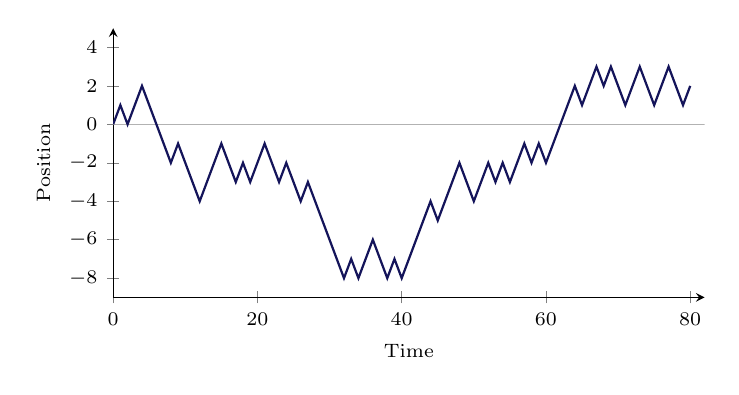
\begin{tikzpicture}[font=\footnotesize]
		\begin{axis}[
				width=0.75\textwidth, height=5.0cm,
				xmin=0, xmax=82, ymin=-9, ymax=5,
				xlabel={Time}, ylabel={Position},
				axis lines=left, axis line style={thin},
				label style={font=\scriptsize}, tick label style={font=\scriptsize},
				xtick={0,20,40,60,80}, ytick={-8,-6,-4,-2,0,2,4},
			]
			\addplot[Gray!60, thin] coordinates {(0,0) (82,0)};
			\addplot[MidnightBlue!80!black, thick] coordinates {(0,0) (1,1) (2,0) (3,1) (4,2) (5,1) (6,0) (7,-1) (8,-2) (9,-1) (10,-2) (11,-3) (12,-4) (13,-3) (14,-2) (15,-1) (16,-2) (17,-3) (18,-2) (19,-3) (20,-2) (21,-1) (22,-2) (23,-3) (24,-2) (25,-3) (26,-4) (27,-3) (28,-4) (29,-5) (30,-6) (31,-7) (32,-8) (33,-7) (34,-8) (35,-7) (36,-6) (37,-7) (38,-8) (39,-7) (40,-8) (41,-7) (42,-6) (43,-5) (44,-4) (45,-5) (46,-4) (47,-3) (48,-2) (49,-3) (50,-4) (51,-3) (52,-2) (53,-3) (54,-2) (55,-3) (56,-2) (57,-1) (58,-2) (59,-1) (60,-2) (61,-1) (62,0) (63,1) (64,2) (65,1) (66,2) (67,3) (68,2) (69,3) (70,2) (71,1) (72,2) (73,3) (74,2) (75,1) (76,2) (77,3) (78,2) (79,1) (80,2)};
		\end{axis}
	\end{tikzpicture}
	\caption{A sample path of the symmetric random walk over 80 steps.}
	\label{fig:random-walk}
\end{figure}

\zh{binomial model 其實就是 random walk：粒子在整數線上，每步以機率 $p$ 往右、$1-p$ 往左一格；$p=1/2$ 時叫 symmetric。和 BOPM 的關係：粒子的位置就是到目前為止上漲次數減下跌次數。}

\begin{remark}
	\textbf{和 BOPM 的對應。}$n$ 步中往右 $j$ 次時位置是 $j-(n-j)=2j-n$；CRR tree（$d=1/u$）中上漲 $j$ 次的股價是 $Su^{j}d^{\,n-j}=Su^{2j-n}$。所以 $\ln(S_{n}/S)=(2j-n)\ln u$：log 股價就是步長 $\ln u$ 的 random walk，$j\sim\mathrm{Bin}(n,p)$。
\end{remark}

\subsection{Random Walk with Drift}

\source{Slide p.~548}

\begin{definition}
	A \vocab{random walk with drift} is
	\[
		X_{n} \;=\; \mu+X_{n-1}+\xi_{n} ,
	\]
	where $\xi_{n}$ are independent and identically distributed with zero mean.
	The \vocab{drift} $\mu$ is the expected change per period.
\end{definition}

Note that this process is continuous in space.

\zh{random walk with drift：$X_{n}=\mu+X_{n-1}+\xi_{n}$，$\xi_{n}$ 是 i.i.d.\ 平均為 $0$ 的隨機變數；drift $\mu$ 是每期的期望變化量。注意這個過程在空間上是連續的（$\xi_{n}$ 可以取任意實數值）。}

%─────§ Martingales──────────────────────────────────────────────────────────────────────────────────────────────────────────────────────────────────
\section{Martingales}
\label{sec:martingales}

\source{Slides pp.~549--550}

\begin{definition}
	$\{X(t),t\ge0\}$ is a \vocab{martingale}\footnote{The origin of the name is somewhat obscure.} if $E[\,\abs{X(t)}\,]<\infty$ for $t\ge0$ and
	\begin{equation}
		E\bigl[\,X(t)\mid X(u),\,0\le u\le s\,\bigr] \;=\; X(s) , \qquad s\le t .
		\label{eq:martingale-ct}
	\end{equation}
	In the discrete-time setting, a martingale means
	\begin{equation}
		E[\,X_{n+1}\mid X_{1},X_{2},\dots,X_{n}\,] \;=\; X_{n} .
		\label{eq:martingale-dt}
	\end{equation}
\end{definition}

$X_{n}$ can be interpreted as a gambler's fortune after the $n$th gamble.
Identity \eqref{eq:martingale-dt} then says the expected fortune after the $(n+1)$st gamble equals the fortune after the $n$th gamble regardless of what may have occurred before.
A martingale is therefore a notion of fair games.

\zh{martingale：$E[\abs{X(t)}]<\infty$ 且給定到 $s$ 為止的整段歷史，$X(t)$ 的條件期望值等於 $X(s)$ \eqref{eq:martingale-ct}；離散版本是 \eqref{eq:martingale-dt}。把 $X_{n}$ 想成賭徒第 $n$ 次賭完的財富，\eqref{eq:martingale-dt} 說不論之前發生什麼，下一把之後的期望財富等於現在的財富，所以 martingale 是「公平賭局」的概念。}

\begin{proposition}
	If $\{X_{n}\}$ is a martingale, then
	\begin{equation}
		E[\,X_{n}\,] \;=\; E[\,X_{1}\,]
		\label{eq:martingale-mean}
	\end{equation}
	for all $n$.
	Similarly, $E[\,X(t)\,]=E[\,X(0)\,]$ in the continuous-time case.
\end{proposition}

\begin{proof}
	Apply the law of iterated conditional expectations \eqref{eq:tower} to both sides of \eqref{eq:martingale-dt}: $E[X_{n+1}]=E\bigl[E[X_{n+1}\mid X_{1},\dots,X_{n}]\bigr]=E[X_{n}]$, and induct on $n$.
\end{proof}

\zh{對 \eqref{eq:martingale-dt} 兩邊取期望值並用 tower law \eqref{eq:tower}，得 $E[X_{n+1}]=E[X_{n}]$，所以 martingale 的期望值永遠不變 \eqref{eq:martingale-mean}。}

\subsection{Still a Martingale?}

\source{Slides pp.~551--553}

Suppose we replace \eqref{eq:martingale-dt} with
\[
	E[\,X_{n+1}\mid X_{n}\,] \;=\; X_{n} .
\]
It also says past history cannot affect the future.
But is it equivalent to the original definition \eqref{eq:martingale-dt}?\footnote{Contributed by Mr.~Hsieh, Chicheng (\texttt{M9007304}) on April 13, 2005.}
Well, no.\footnote{Contributed by Mr.~Zhang, Ann-Sheng (\texttt{B89201033}) on April 13, 2005.}
The slides consider this random walk with drift:
\[
	X_{i} \;=\;
	\begin{cases}
		X_{i-1}+\xi_{i} , & \text{if $i$ is even}, \\
		X_{i-2} ,         & \text{otherwise},
	\end{cases}
\]
where $\xi_{n}$ are random variables with zero mean, and claim that
\[
	E[\,X_{i}\mid X_{i-1}\,] \;=\;
	\begin{cases}
		X_{i-1} , & \text{if $i$ is even}, \\
		X_{i-1} , & \text{otherwise},
	\end{cases}
\]
so it is a martingale by the ``new'' definition.
But
\[
	E[\,X_{i}\mid\dots,X_{i-2},X_{i-1}\,] \;=\;
	\begin{cases}
		X_{i-1} , & \text{if $i$ is even}, \\
		X_{i-2} , & \text{otherwise},
	\end{cases}
\]
so it is not a martingale by the original definition.

\zh{若把 \eqref{eq:martingale-dt} 改成只對前一期取條件 $E[X_{n+1}\mid X_{n}]=X_{n}$，它看起來也說「過去不影響未來」，但和原定義不等價。簡報的例子：$i$ 為偶數時 $X_{i}=X_{i-1}+\xi_{i}$，奇數時 $X_{i}=X_{i-2}$；簡報說它在新定義下是 martingale，但給定整段歷史時，奇數 $i$ 的條件期望是 $X_{i-2}\ne X_{i-1}$，所以不是原定義的 martingale。}

\begin{note}
	簡報這個例子的「新定義」那一半其實不成立（只要 $\xi$ 不是 $0$ 且變異數有限）。奇數 $i$ 時 $X_{i}=X_{i-2}=X_{i-1}-\xi_{i-1}$，所以
	\[
		E[\,X_{i}\mid X_{i-1}\,] \;=\; X_{i-1}-E[\,\xi_{i-1}\mid X_{i-1}\,] ,
	\]
	要等於 $X_{i-1}$ 必須 $E[\xi_{i-1}\mid X_{i-2}+\xi_{i-1}]=0$。下面的 lemma 說這只有在 $\xi_{i-1}=0$ 時才可能。
\end{note}

\begin{lemma}
	\label{lem:two-way-martingale}
	Let $Y,Z$ have finite second moments.
	If $E[Z\mid Y]=Y$ and $E[Y\mid Z]=Z$, then $Y=Z$ with probability one.
\end{lemma}

\begin{proof}
	由 \autoref{prop:ce-properties}(2)（已知的 $Y$ 可以提出來；$Y$ 不必有界，因為由 \autoref{lem:cauchy-schwarz}，$YZ$ 可積）與 tower law \eqref{eq:tower}，$E[YZ]=E\bigl[Y\,E[Z\mid Y]\bigr]=E[Y^{2}]$；對稱地 $E[YZ]=E[Z^{2}]$。所以 $E[(Z-Y)^{2}]=E[Z^{2}]-2E[YZ]+E[Y^{2}]=0$，由 \autoref{lem:zero-mean}，$Z-Y=0$ with probability one。
\end{proof}

套在簡報的例子：$Y=X_{i-2}$、$Z=X_{i-1}=X_{i-2}+\xi_{i-1}$。偶數步的條件 $E[\xi_{i-1}\mid X_{i-2}]=0$ 給 $E[Z\mid Y]=Y$；若奇數步也滿足新定義就是 $E[Y\mid Z]=Z$，於是 $\xi_{i-1}=0$，整個過程是常數。一個真正的反例：
\begin{eg}[補充]
	$X_{1}\in\{-1,1\}$、$\xi_{2}\in\{-1,1\}$ 獨立、各機率 $1/2$，$X_{2}=X_{1}+\xi_{2}\in\{-2,0,2\}$，令
	\[
		X_{3} \;=\;
		\begin{cases}
			X_{1} , & X_{2}=0 , \\
			X_{2} , & X_{2}=\pm2 .
		\end{cases}
	\]
	\begin{enumerate}[(1),nosep]
		\item $E[X_{2}\mid X_{1}]=X_{1}+E[\xi_{2}]=X_{1}$。
		\item $X_{2}=\pm2$ 時 $X_{3}=X_{2}$；$X_{2}=0$ 時 $(X_{1},\xi_{2})=(1,-1)$ 或 $(-1,1)$ 等機率，$E[X_{3}\mid X_{2}=0]=E[X_{1}\mid X_{2}=0]=0=X_{2}$。所以 $E[X_{3}\mid X_{2}]=X_{2}$，新定義成立。
		\item 但 $E[X_{3}\mid X_{1},X_{2}=0]=X_{1}=\pm1\ne0=X_{2}$，原定義 \eqref{eq:martingale-dt} 不成立。
	\end{enumerate}
\end{eg}

新定義只看 $X_{2}$，看不出 $X_{2}=0$ 是怎麼來的；完整歷史知道 $X_{1}$，就能預測 $X_{3}$ 的方向。

\source{Slide p.~554}

\begin{eg}
	\label{eg:sum-martingale}
	Consider the stochastic process $\{Z_{n}\triangleq\sum_{i=1}^{n}X_{i},\ n\ge1\}$, where $X_{i}$ are independent random variables with zero mean.
	This process is a martingale because
	\begin{align*}
		E[\,Z_{n+1}\mid Z_{1},Z_{2},\dots,Z_{n}\,]
		& \;=\; E[\,Z_{n}+X_{n+1}\mid Z_{1},Z_{2},\dots,Z_{n}\,] \\
		& \;=\; E[\,Z_{n}\mid Z_{1},Z_{2},\dots,Z_{n}\,]+E[\,X_{n+1}\mid Z_{1},Z_{2},\dots,Z_{n}\,] \\
		& \;=\; Z_{n}+E[\,X_{n+1}\,] \;=\; Z_{n} .
	\end{align*}
\end{eg}

\zh{例：$Z_{n}=\sum_{i=1}^{n}X_{i}$，$X_{i}$ 獨立且平均為 $0$，則 $\{Z_{n}\}$ 是 martingale。}

\begin{remark}
	最後一行用了兩件事：$Z_{n}$ 是已知的，條件期望就是它自己；$X_{n+1}$ 和 $X_{1},\dots,X_{n}$ 獨立，而 $Z_{1},\dots,Z_{n}$ 只是 $X_{1},\dots,X_{n}$ 的函數，所以條件期望等於無條件期望 $E[X_{n+1}]=0$（\autoref{prop:ce-properties}）。
\end{remark}

\subsection{Probability Measure}
\label{sec:probability-measure}

\source{Slides pp.~555--557}

A \vocab{probability measure} assigns probabilities to states of the world.\footnote{Only certain sets such as the Borel sets receive probabilities (Feller, 1972).}
A martingale is defined with respect to a probability measure, under which the expectation is taken.
Second, a martingale is defined with respect to an \vocab{information set}.
In the characterizations \eqref{eq:martingale-ct}--\eqref{eq:martingale-dt}, the information set contains the current and past values of $X$ by default, but it need not be so.

\zh{probability measure 指定各個 state 的機率。martingale 是相對於某個 probability measure（期望值在它之下取）、以及某組 information set 來定義的。\eqref{eq:martingale-ct}--\eqref{eq:martingale-dt} 預設 information set 是 $X$ 現在和過去的值，但不一定要如此。}

\begin{definition}
	A stochastic process $\{X(t),t\ge0\}$ is a martingale with respect to information sets $\{I_{t}\}$ if, for all $t\ge0$, $E[\,\abs{X(t)}\,]<\infty$ and
	\[
		E[\,X(u)\mid I_{t}\,] \;=\; X(t)
	\]
	for all $u>t$.
	The discrete-time version: for all $n>0$, $E[\,X_{n+1}\mid I_{n}\,]=X_{n}$, given the information sets $\{I_{n}\}$.
\end{definition}

The above implies
\[
	E[\,X_{n+m}\mid I_{n}\,] \;=\; X_{n}
\]
for any $m>0$ by \eqref{eq:tower-nested}.
A typical $I_{n}$ is the price information up to time $n$.
Then the above identity says the FVs of $X$ will not deviate systematically from today's value given the price history.

\zh{相對於 information sets $\{I_{t}\}$ 的 martingale：$E[X(u)\mid I_{t}]=X(t)$，$u>t$；離散版 $E[X_{n+1}\mid I_{n}]=X_{n}$。由 \eqref{eq:tower-nested} 可推出 $E[X_{n+m}\mid I_{n}]=X_{n}$。$I_{n}$ 通常是到時間 $n$ 為止的價格資訊，這時上式說：給定價格歷史，$X$ 的未來值不會系統性地偏離今天的值。}

\begin{remark}
	\textbf{$E[X_{n+m}\mid I_{n}]=X_{n}$ 怎麼來。}對 $m$ 歸納：$I_{n}\subseteq I_{n+m-1}$（資訊只會累積），由 \eqref{eq:tower-nested}，
	\[
		E[\,X_{n+m}\mid I_{n}\,] \;=\; E\bigl[\,E[\,X_{n+m}\mid I_{n+m-1}\,]\mid I_{n}\,\bigr] \;=\; E[\,X_{n+m-1}\mid I_{n}\,] \;=\; X_{n} ,
	\]
	中間用了一步的 martingale 性質，最後一步是歸納假設。
\end{remark}

\source{Slides pp.~558--559}

\begin{eg}
	Consider the stochastic process $\{Z_{n}-n\mu,\ n\ge1\}$, where $Z_{n}\triangleq\sum_{i=1}^{n}X_{i}$ and $X_{1},X_{2},\dots$ are independent random variables with mean $\mu$.
	Now,
	\begin{align*}
		E[\,Z_{n+1}-(n+1)\mu\mid X_{1},X_{2},\dots,X_{n}\,]
		& \;=\; E[\,Z_{n+1}\mid X_{1},X_{2},\dots,X_{n}\,]-(n+1)\mu \\
		& \;=\; E[\,Z_{n}+X_{n+1}\mid X_{1},X_{2},\dots,X_{n}\,]-(n+1)\mu \\
		& \;=\; Z_{n}+\mu-(n+1)\mu \\
		& \;=\; Z_{n}-n\mu .
	\end{align*}
	Define $I_{n}\triangleq\{X_{1},X_{2},\dots,X_{n}\}$.
	Then $\{Z_{n}-n\mu,\ n\ge1\}$ is a martingale with respect to $\{I_{n}\}$.
\end{eg}

\zh{例：$X_{i}$ 獨立、平均 $\mu$，$Z_{n}=\sum_{i=1}^{n}X_{i}$。扣掉 drift 後 $\{Z_{n}-n\mu\}$ 是相對於 $I_{n}=\{X_{1},\dots,X_{n}\}$ 的 martingale。注意 information set 是 $X_{i}$ 而不是過程本身的值。}

%─────§ Martingale pricing───────────────────────────────────────────────────────────────────────────────────────────────────────────────────────────
\section{Martingale Pricing}
\label{sec:martingale-pricing}

\source{Slides pp.~560--561}

Stock prices and zero-coupon bond prices are expected to rise, while call prices are expected to fall (\autoref{sec:theta}).
They are not martingales.
Why is then martingale useful?
Recall a martingale is defined with respect to some information set and some probability measure.
By modifying the probability measure, we can convert a price process into a martingale.

\zh{股價和 zero-coupon bond 價格預期會上漲，call 價格預期會下跌（theta），它們都不是 martingale。那 martingale 有什麼用？martingale 是相對於某個 information set 和 probability measure 定義的；換掉 probability measure，就能把價格過程變成 martingale。}

The price of a European option is the expected discounted payoff in a risk-neutral economy \eqref{eq:rn-pricing}.
This principle can be generalized using the concept of martingale.
Recall the recursive valuation of European option via \eqref{eq:bopm-expectation}:
\[
	C \;=\; \bigl[\,pC_{u}+(1-p)\,C_{d}\,\bigr]/R ,
\]
where $p$ is the risk-neutral probability and \$1 grows to \$$R$ in a period.

\zh{European option 的價格是 risk-neutral 下 payoff 折現的期望值 \eqref{eq:rn-pricing}，這可以用 martingale 推廣。回憶一期的遞迴 $C=[pC_{u}+(1-p)C_{d}]/R$。}

\source{Slides pp.~562--563}

Let $C(i)$ denote the value of the option at time $i$.
Consider the discount process
\[
	\bigl\{\,C(i)/R^{i},\ i=0,1,\dots,n\,\bigr\} .
\]
Then,
\[
	E\left[\,\frac{C(i+1)}{R^{i+1}}\;\middle|\;S(i)\,\right]
	\;=\; \frac{E[\,C(i+1)\mid S(i)\,]}{R^{i+1}}
	\;=\; \frac{pC_{u}+(1-p)\,C_{d}}{R^{i+1}}
	\;=\; \frac{C(i)}{R^{i}} .
\]
It is easy to generalize it to
\[
	E\left[\,\frac{C(k)}{R^{k}}\;\middle|\;S(i)\,\right] \;=\; \frac{C(i)}{R^{i}} , \qquad i\le k .
\]

\zh{令 $C(i)$ 為 option 在時間 $i$ 的價值，考慮折現過程 $C(i)/R^{i}$。在 risk-neutral 機率下，給定 $S(i)$ 時下一期折現值的期望等於這一期的折現值，再推廣到任意 $k\ge i$。}

\begin{remark}
	\begin{enumerate}[(1),nosep]
		\item \textbf{第二個等號。}給定 $S(i)$，$C(i+1)$ 以機率 $p$ 是 $C_{u}$、以 $1-p$ 是 $C_{d}$（$C_{u},C_{d}$ 是 $S(i)$ 往上、往下那兩個 node 的值）。
		\item \textbf{第三個等號。}由 \eqref{eq:bopm-expectation}，$pC_{u}+(1-p)C_{d}=RC(i)$，除以 $R^{i+1}$ 得 $C(i)/R^{i}$。
		\item \textbf{推廣到 $k$。}和上面 $E[X_{n+m}\mid I_{n}]=X_{n}$ 的 remark 相同，用 \eqref{eq:tower-nested} 一步一步往回推。
	\end{enumerate}
	要注意期望值是在 risk-neutral 機率 $p$ 下取的：真實機率下 $C(i)/R^{i}$ 不是 martingale。
\end{remark}

This simplified formulation assumes:\footnote{Contributed by Mr.~Wang, Liang-Kai (Ph.D.\ student, ECE, University of Wisconsin-Madison) and Mr.~Hsiao, Huan-Wen (\texttt{B90902081}) on May 3, 2006.}
\begin{enumerate}[(1),nosep]
	\item The model is Markovian: the distribution of the future is determined by the present (time $i$) and not the past.
	\item The payoff depends only on the terminal price of the underlying asset (Asian options do not qualify); recall they are called simple claims (\autoref{sec:path-dependent}).
\end{enumerate}

\zh{這個簡化版本假設 (1) 模型是 Markovian：未來的分布只由現在決定，與過去無關；(2) payoff 只取決於標的的最終價格（simple claim），Asian option 不符合。}

In general, the discount process is a martingale in that\footnote{In this general formulation, Asian options do qualify.}
\begin{equation}
	E_{i}^{\pi}\left[\,\frac{C(k)}{R^{k}}\,\right] \;=\; \frac{C(i)}{R^{i}} , \qquad i\le k ,
	\label{eq:martingale-pricing}
\end{equation}
where $E_{i}^{\pi}$ is taken under the risk-neutral probability conditional on the price information up to time $i$.
This risk-neutral probability is also called the EMM, or the \vocab{equivalent martingale (probability) measure}.\footnote{Two probability measures are said to be equivalent if they assign nonzero probabilities to the same set of states.}

\zh{一般情形下，折現過程在 risk-neutral 機率下、相對於到時間 $i$ 為止的價格資訊是 martingale \eqref{eq:martingale-pricing}（這個版本 Asian option 也適用）。這個 risk-neutral 機率又叫 EMM（equivalent martingale measure）；兩個 probability measure equivalent 指它們給正機率的 state 集合相同。}

\begin{remark}
	\textbf{為什麼一般版本 Asian option 也可以。}簡化版只以 $S(i)$ 為條件，但 Asian option 在時間 $i$ 的價值還取決於到目前為止的平均價，光知道 $S(i)$ 不夠。$E_{i}^{\pi}$ 以完整的價格歷史為條件，平均價也包含在內，所以 $C(i)$ 是這份資訊的函數，遞迴照樣成立。
\end{remark}

\source{Slides pp.~564--566}

Equation \eqref{eq:martingale-pricing} holds for all assets, not just options.
When interest rates are stochastic, the equation becomes
\begin{equation}
	\frac{C(i)}{M(i)} \;=\; E_{i}^{\pi}\left[\,\frac{C(k)}{M(k)}\,\right] , \qquad i\le k ,
	\label{eq:martingale-pricing-M}
\end{equation}
where $M(j)$ is the balance in the money market account at time $j$ using the rollover strategy with an initial investment of \$1.
It is called the \vocab{bank account process}.
It says the discount process is a martingale under $\pi$.
If interest rates are stochastic, then $M(j)$ is a random variable: $M(0)=1$, and $M(j)$ is known at time $j-1$ because the interest rate for the next period has been revealed then.
Identity \eqref{eq:martingale-pricing-M} is the general formulation of risk-neutral valuation.

\zh{\eqref{eq:martingale-pricing} 對所有資產都成立。利率是隨機時改寫成 \eqref{eq:martingale-pricing-M}，$M(j)$ 是期初投入 \$1、每期滾存在貨幣市場帳戶的餘額（bank account process）。$M(j)$ 是隨機變數，$M(0)=1$，且在 $j-1$ 時就已知（下一期利率已揭露）。\eqref{eq:martingale-pricing-M} 是 risk-neutral valuation 的一般形式。}

\begin{remark}
	\begin{enumerate}[(1),nosep]
		\item \textbf{$M(j)$。}記 $r_{\ell}$ 為第 $\ell$ 期（從 $\ell$ 到 $\ell+1$）的利率，在時間 $\ell$ 揭露，則 $M(j)=\prod_{\ell=0}^{j-1}(1+r_{\ell})$（連續複利則是 $e^{\sum r_{\ell}}$）。最後一個因子 $1+r_{j-1}$ 在 $j-1$ 已知，所以 $M(j)$ 在 $j-1$ 已知。
		\item \textbf{和 \eqref{eq:martingale-pricing} 的關係。}利率固定時 $M(j)=R^{j}$，\eqref{eq:martingale-pricing-M} 就是 \eqref{eq:martingale-pricing}。
		\item \textbf{定價怎麼用。}取 $i=0$、$k=n$：$C(0)=E^{\pi}\bigl[C(n)/M(n)\bigr]$，就是把到期 payoff 沿著實際走過的利率路徑折現，再取 risk-neutral 期望。$M(n)$ 隨機時不能拆成 $E^{\pi}[C(n)]/M(n)$。
	\end{enumerate}
\end{remark}

\source{Slide p.~567}

\begin{theorem}
	\label{thm:ftap}
	A discrete-time model is arbitrage-free if and only if there exists an equivalent probability measure (the risk-neutral probability measure) such that the discount process is a martingale.
\end{theorem}

\zh{離散時間模型沒有套利，若且唯若存在一個 equivalent probability measure（risk-neutral 機率），使折現過程是 martingale。}

\begin{note}
	這是 \vocab{fundamental theorem of asset pricing}（Harrison \& Pliska, 1981）。在一期 BOPM 中就是 \autoref{sec:pseudo-prob} 的結論：$p=\frac{R-d}{u-d}\in(0,1)$ 若且唯若 $d<R<u$，而 $R\le d$ 或 $R\ge u$ 時分別借錢買股票、放空股票存錢就是套利。「equivalent」要求每個真實可能發生的 state 在 $\pi$ 下機率也大於 $0$，即 $p\ne0,1$。
\end{note}

\subsection{Futures Price under the BOPM}

\source{Slides pp.~568--569}

Futures prices form a martingale under the risk-neutral probability $p_{f}$ \eqref{eq:pf}.
The expected futures price in the next period is
\[
	p_{f}Fu+(1-p_{f})\,Fd \;=\; F\left(\frac{1-d}{u-d}\,u+\frac{u-1}{u-d}\,d\right) \;=\; F .
\]
This can be generalized to
\[
	F_{i} \;=\; E_{i}^{\pi}[\,F_{k}\,] , \qquad i\le k ,
\]
where $F_{i}$ is the futures price at time $i$.
This equation holds under stochastic interest rates, too.\footnote{See Exercise 13.2.11 of the textbook.}

\zh{futures price 在 $p_{f}$ 下是 martingale：下一期期望值 $p_{f}Fu+(1-p_{f})Fd=F$，推廣到 $F_{i}=E_{i}^{\pi}[F_{k}]$，利率隨機時也成立。}

\begin{remark}
	括號內 $\frac{(1-d)u+(u-1)d}{u-d}=\frac{u-ud+ud-d}{u-d}=1$。注意 futures price 本身（不折現）就是 martingale，因為持有 futures 部位不用花錢，沒有需要賺到 $R$ 的本金。
\end{remark}

Futures prices do not form a martingale under the risk-neutral probability $p=(R-d)/(u-d)$ \eqref{eq:risk-neutral-p}.
The expected futures price in the next period equals
\[
	Fu\,\frac{R-d}{u-d}+Fd\,\frac{u-R}{u-d}
	\;=\; F\,\frac{uR-ud}{u-d}+F\,\frac{ud-Rd}{u-d}
	\;=\; FR .
\]
But they do if $u$ and $d$ are changed to $u/R$ and $d/R$, respectively, justified by \eqref{eq:fwd-price}.

\zh{在股票的 risk-neutral 機率 $p=(R-d)/(u-d)$ 下，若讓 futures price 也乘 $u$、$d$，期望值是 $FR$，不是 martingale。但 futures price 的乘數其實應該是 $u/R$、$d/R$（由 \eqref{eq:fwd-price}），這時就是 martingale。}

\begin{remark}
	\textbf{為什麼是 $u/R$、$d/R$。}股價從 $S$ 漲到 $Su$ 時，由 \eqref{eq:fwd-price}，futures price 從 $F=Se^{rT}$ 變成 $Sue^{r(T-\Delta t)}=Fu/R$（$R=e^{r\Delta t}$）：剩餘期限少了一期，少乘一個 $R$。於是期望值 $p\,Fu/R+(1-p)\,Fd/R=FR/R=F$。
	這和 \eqref{eq:pf} 是同一件事的兩種寫法：futures price 用乘數 $u,d$ 配 $p_{f}$，或股價用乘數 $u,d$、futures price 用 $u/R,d/R$ 配 $p$。
\end{remark}

\subsection{Martingale Pricing and Numeraire}
\label{sec:numeraire}

\source{Slides pp.~570--571}

The martingale pricing formula \eqref{eq:martingale-pricing-M} uses the money market account as \vocab{numeraire}:\footnote{John Law (1671--1729): ``Money to be qualified for exchanging goods and for payments need not be certain in its value.''} it expresses the price of any asset relative to the money market account.\footnote{Leon Walras (1834--1910).}
The money market account is not the only choice for numeraire.
Suppose asset $S$'s value is positive at all time, and choose $S$ as numeraire.
Martingale pricing says there exists a risk-neutral probability $\pi$ under which the relative price of any asset $C$ is a martingale:
\[
	\frac{C(i)}{S(i)} \;=\; E_{i}^{\pi}\left[\,\frac{C(k)}{S(k)}\,\right] , \qquad i\le k ,
\]
where $S(j)$ denotes the price of $S$ at time $j$.
So the ``discount'' process remains a martingale.\footnote{This result is related to Girsanov's theorem (1960).}

\zh{\eqref{eq:martingale-pricing-M} 以貨幣市場帳戶為 numeraire（計價單位），把每個資產的價格表示成相對於它的比值。numeraire 不必是貨幣市場帳戶：任何價格永遠為正的資產 $S$ 都可以，此時存在某個 risk-neutral 機率 $\pi$，使任何資產相對於 $S$ 的價格 $C/S$ 是 martingale。}

\source{Slides pp.~572--576}

\begin{eg}
	\label{eg:numeraire}
	Take the binomial model with two assets.
	In a period, asset one's price can go from $S$ to $S_{1}$ or $S_{2}$; asset two's price can go from $P$ to $P_{1}$ or $P_{2}$.
	Both assets must move up or down at the same time.
	Assume
	\begin{equation}
		\frac{S_{1}}{P_{1}} \;<\; \frac{S}{P} \;<\; \frac{S_{2}}{P_{2}}
		\label{eq:numeraire-no-arb}
	\end{equation}
	to rule out arbitrage opportunities.

	For any derivative security, let $C_{1}$ be its price at time one if asset one's price moves to $S_{1}$, and $C_{2}$ if it moves to $S_{2}$.
	Replicate the derivative by solving
	\begin{align*}
		\alpha S_{1}+\beta P_{1} & \;=\; C_{1} , \\
		\alpha S_{2}+\beta P_{2} & \;=\; C_{2} ,
	\end{align*}
	using $\alpha$ units of asset one and $\beta$ units of asset two.
	By \eqref{eq:numeraire-no-arb}, $\alpha$ and $\beta$ have unique solutions:
	\[
		\alpha \;=\; \frac{P_{2}C_{1}-P_{1}C_{2}}{P_{2}S_{1}-P_{1}S_{2}}
		\qquad\text{and}\qquad
		\beta \;=\; \frac{S_{2}C_{1}-S_{1}C_{2}}{S_{2}P_{1}-S_{1}P_{2}} .
	\]
	The derivative costs
	\[
		C \;=\; \alpha S+\beta P \;=\; \frac{P_{2}S-PS_{2}}{P_{2}S_{1}-P_{1}S_{2}}\,C_{1}+\frac{PS_{1}-P_{1}S}{P_{2}S_{1}-P_{1}S_{2}}\,C_{2} .
	\]
	It is easy to verify that
	\begin{equation}
		\frac{C}{P} \;=\; p\,\frac{C_{1}}{P_{1}}+(1-p)\,\frac{C_{2}}{P_{2}}
		\qquad\text{with}\qquad
		p \;\triangleq\; \frac{(S/P)-(S_{2}/P_{2})}{(S_{1}/P_{1})-(S_{2}/P_{2})} .
		\label{eq:numeraire-p}
	\end{equation}
	By \eqref{eq:numeraire-no-arb}, $0<p<1$.
	$C$'s price using asset two as numeraire (i.e., $C/P$) is a martingale under the risk-neutral probability $p$.
	The expected returns of the two assets are irrelevant.
\end{eg}

\zh{例：兩個資產的一期 binomial model，資產一從 $S$ 變成 $S_{1}$ 或 $S_{2}$，資產二從 $P$ 變成 $P_{1}$ 或 $P_{2}$，同漲同跌；\eqref{eq:numeraire-no-arb} 排除套利。用 $\alpha$ 單位資產一、$\beta$ 單位資產二複製衍生性商品，解出 $\alpha,\beta$ 並得到價格 $C$。可以驗證 $C/P$ 是 $C_{1}/P_{1}$、$C_{2}/P_{2}$ 以 $p$ \eqref{eq:numeraire-p} 加權的平均，且 $0<p<1$：以資產二為 numeraire，$C/P$ 在 $p$ 下是 martingale。兩個資產的期望報酬無關緊要。}

\begin{remark}
	\begin{enumerate}[(1),nosep]
		\item \textbf{為什麼解唯一。}係數行列式 $S_{1}P_{2}-S_{2}P_{1}=P_{1}P_{2}\bigl(\frac{S_{1}}{P_{1}}-\frac{S_{2}}{P_{2}}\bigr)$，由 \eqref{eq:numeraire-no-arb} 是負的、不為 $0$，用 Cramer's rule 得 $\alpha,\beta$。
		\item \textbf{驗證 \eqref{eq:numeraire-p}。}把 $C$ 除以 $P$，$C_{1}$ 的係數是 $\frac{P_{2}S-PS_{2}}{P(P_{2}S_{1}-P_{1}S_{2})}$；分子分母同除 $P_{2}$ 再乘 $P_{1}$，等於 $\frac{1}{P_{1}}\cdot\frac{S/P-S_{2}/P_{2}}{S_{1}/P_{1}-S_{2}/P_{2}}=\frac{p}{P_{1}}$。$C_{2}$ 的係數同理是 $\frac{1-p}{P_{2}}$。
		\item \textbf{$0<p<1$。}$p$ 的分子 $S/P-S_{2}/P_{2}<0$、分母 $S_{1}/P_{1}-S_{2}/P_{2}<0$，且分子絕對值比分母小（因 $S/P>S_{1}/P_{1}$），所以 $0<p<1$。
		\item \textbf{\eqref{eq:numeraire-no-arb} 為什麼排除套利。}以 $P$ 為單位，資產一的相對價格從 $S/P$ 變成 $S_{1}/P_{1}$ 或 $S_{2}/P_{2}$；若 $S/P$ 不夾在中間，例如 $S/P\le S_{1}/P_{1}<S_{2}/P_{2}$，那麼賣 $S/P$ 單位資產二、買 $1$ 單位資產一，期初成本 $0$，期末 $S_{j}-\frac{S}{P}P_{j}=P_{j}\bigl(\frac{S_{j}}{P_{j}}-\frac{S}{P}\bigr)\ge0$ 且不全為 $0$，是套利。
	\end{enumerate}
\end{remark}

In the BOPM, $S$ is the stock and $P$ is the bond.
Furthermore, $p$ assumes the bond is the numeraire.
In the binomial option pricing formula \eqref{eq:bopm-formula}, $S\sum b(j;n,pu/R)$ uses stock as the numeraire: its probability measure $pu/R$ differs from $p$, and its price at maturity is simply $S$.
$SN(x)$ for the call and $SN(-x)$ for the put in the Black--Scholes formulas (\autoref{thm:black-scholes}) use stock as the numeraire as well.\footnote{See Exercise 13.2.12 of the textbook.}

\zh{在 BOPM 中 $S$ 是股票、$P$ 是債券，$p$ 是以債券為 numeraire 的機率。binomial 公式 \eqref{eq:bopm-formula} 中 $S\sum b(j;n,pu/R)$ 是以股票為 numeraire：機率是 $pu/R$ 而不是 $p$，而 numeraire 本身到期的「價格」就是 $S$。Black--Scholes 公式中 call 的 $SN(x)$ 和 put 的 $SN(-x)$ 也是以股票為 numeraire。}

\begin{remark}
	\textbf{驗證 $pu/R$ 就是以股票為 numeraire 的機率。}在 \eqref{eq:numeraire-p} 中交換兩個資產的角色：資產二換成股票（$P\to S$、$P_{1}\to Su$、$P_{2}\to Sd$），資產一換成債券（$S\to1$、$S_{1},S_{2}\to R$）。則
	\[
		p' \;=\; \frac{1/S-R/(Sd)}{R/(Su)-R/(Sd)} \;=\; \frac{ud-Ru}{Rd-Ru} \;=\; \frac{u(R-d)}{R(u-d)} \;=\; \frac{pu}{R} .
	\]
	所以 \eqref{eq:bopm-formula} 的第一項 $S\sum_{j\ge a}b(j;n,pu/R)$ 是「股票在 $S_{n}\ge X$ 時的價值」：以股票為單位，這個 claim 到期值 $\mathbf{1}_{\{S_{n}\ge X\}}$，今天值 $\mathrm{Prob}'[S_{n}\ge X]$，換回金額再乘 $S$。
\end{remark}

%─────§ Brownian motion──────────────────────────────────────────────────────────────────────────────────────────────────────────────────────────────
\section{Brownian Motion}
\label{sec:brownian-motion}

\source{Slides pp.~577--578}

\begin{definition}
	\vocab{Brownian motion} is a stochastic process $\{X(t),t\ge0\}$ with the following properties.\footnote{Robert Brown (1773--1858).}
	\begin{enumerate}[(1),nosep]
		\item $X(0)=0$, unless stated otherwise.
		\item For any $0\le t_{0}<t_{1}<\cdots<t_{n}$, the random variables $X(t_{k})-X(t_{k-1})$ for $1\le k\le n$ are independent.\footnote{So $X(t)-X(s)$ is independent of $X(r)$ for $r\le s<t$.}
		\item For $0\le s<t$, $X(t)-X(s)\sim N\bigl(\mu(t-s),\ \sigma^{2}(t-s)\bigr)$, where $\mu$ and $\sigma\ne0$ are real numbers.
	\end{enumerate}
\end{definition}

The existence and uniqueness of such a process is guaranteed by Wiener's theorem.\footnote{Norbert Wiener (1894--1964). He received his Ph.D.\ from Harvard in 1912.}
This process will be called a \vocab{$(\mu,\sigma)$ Brownian motion} with drift $\mu$ and variance $\sigma^{2}$.
Although Brownian motion is a continuous function of $t$ with probability one, it is almost nowhere differentiable.
The $(0,1)$ Brownian motion is called the \vocab{Wiener process}.
If condition (3) is replaced by ``$X(t)-X(s)$ depends only on $t-s$,'' we have the more general \vocab{L\'evy process}.\footnote{Paul L\'evy (1886--1971).}

\zh{Brownian motion：(1) $X(0)=0$；(2) 不重疊區間的增量互相獨立；(3) $X(t)-X(s)\sim N(\mu(t-s),\sigma^{2}(t-s))$，$\sigma\ne0$。Wiener 定理保證這種過程存在且唯一，叫做 drift $\mu$、variance $\sigma^{2}$ 的 $(\mu,\sigma)$ Brownian motion。它以機率 1 是 $t$ 的連續函數，但幾乎處處不可微。$(0,1)$ Brownian motion 叫 Wiener process。若 (3) 只要求增量的分布只取決於 $t-s$，就是更一般的 Lévy process。}

\source{Slide p.~579}

\begin{eg}
	If $\{X(t),t\ge0\}$ is the Wiener process, then $X(t)-X(s)\sim N(0,t-s)$.
	A $(\mu,\sigma)$ Brownian motion $Y=\{Y(t),t\ge0\}$ can be expressed in terms of the Wiener process:
	\begin{equation}
		Y(t) \;=\; \mu t+\sigma X(t) .
		\label{eq:bm-wiener}
	\end{equation}
	Note that $Y(t+s)-Y(t)\sim N(\mu s,\sigma^{2}s)$.
\end{eg}

\zh{例：Wiener process 的增量 $X(t)-X(s)\sim N(0,t-s)$；任何 $(\mu,\sigma)$ Brownian motion 都可以寫成 $Y(t)=\mu t+\sigma X(t)$ \eqref{eq:bm-wiener}，其增量 $Y(t+s)-Y(t)\sim N(\mu s,\sigma^{2}s)$。}

\begin{remark}
	$Y(t+s)-Y(t)=\mu s+\sigma\bigl(X(t+s)-X(t)\bigr)$，而 $X(t+s)-X(t)\sim N(0,s)$；常數平移 $\mu s$、乘上 $\sigma$ 後仍是 normal（\autoref{cor:normal-closure}），平均 $\mu s$、變異數 $\sigma^{2}s$。獨立增量也直接繼承自 $X$。
\end{remark}

\subsection{Brownian Motion as Limit of Random Walk}

\source{Slides pp.~580--583}

\begin{proposition}
	\label{prop:bm-limit}
	A $(\mu,\sigma)$ Brownian motion is the limiting case of random walk.
\end{proposition}

A particle moves $\Delta x$ to the right with probability $p$ after $\Delta t$ time, and $\Delta x$ to the left with probability $1-p$.
Define
\[
	X_{i} \;\triangleq\;
	\begin{cases}
		+1 , & \text{if the $i$th move is to the right}, \\
		-1 , & \text{if the $i$th move is to the left}.
	\end{cases}
\]
$X_{i}$ are independent with $\mathrm{Prob}[X_{i}=1]=p=1-\mathrm{Prob}[X_{i}=-1]$.
Recall
\[
	E[\,X_{i}\,] \;=\; 2p-1 ,
	\qquad
	\Var[\,X_{i}\,] \;=\; 1-(2p-1)^{2} .
\]
Assume $n\triangleq t/\Delta t$ is an integer.
The particle's position at time $t$ is
\[
	Y(t) \;\triangleq\; \Delta x\,(X_{1}+X_{2}+\cdots+X_{n}) .
\]
Therefore,
\begin{align*}
	E[\,Y(t)\,]   & \;=\; n\,(\Delta x)\,(2p-1) ,               \\
	\Var[\,Y(t)\,] & \;=\; n\,(\Delta x)^{2}\bigl[\,1-(2p-1)^{2}\,\bigr] .
\end{align*}
With $\Delta x\triangleq\sigma\sqrt{\Delta t}$ and $p\triangleq\bigl[\,1+(\mu/\sigma)\sqrt{\Delta t}\,\bigr]/2$ --- identical to \eqref{eq:crr} ---
\begin{align*}
	E[\,Y(t)\,]   & \;=\; n\sigma\sqrt{\Delta t}\,(\mu/\sigma)\sqrt{\Delta t} \;=\; \mu t ,                          \\
	\Var[\,Y(t)\,] & \;=\; n\sigma^{2}\Delta t\,\bigl[\,1-(\mu/\sigma)^{2}\Delta t\,\bigr] \;\to\; \sigma^{2}t ,
\end{align*}
as $\Delta t\to0$.
Thus, $\{Y(t),t\ge0\}$ converges to a $(\mu,\sigma)$ Brownian motion by the central limit theorem (\autoref{thm:clt}).

\zh{粒子每 $\Delta t$ 時間以機率 $p$ 往右、$1-p$ 往左移 $\Delta x$；$X_{i}=\pm1$ 記錄第 $i$ 步方向，彼此獨立。時間 $t$ 的位置 $Y(t)=\Delta x(X_{1}+\cdots+X_{n})$，$n=t/\Delta t$。取 $\Delta x=\sigma\sqrt{\Delta t}$、$p=[1+(\mu/\sigma)\sqrt{\Delta t}]/2$（和 \eqref{eq:crr} 相同），則 $E[Y(t)]=\mu t$、$\Var[Y(t)]\to\sigma^{2}t$，由 central limit theorem，$Y$ 收斂到 $(\mu,\sigma)$ Brownian motion。}

\begin{remark}
	\begin{enumerate}[(1),nosep]
		\item \textbf{$X_{i}$ 的動差。}$E[X_{i}]=p-(1-p)=2p-1$；$X_{i}^{2}=1$，所以 $\Var[X_{i}]=1-(2p-1)^{2}$。
		\item \textbf{$Y(t)$ 的動差。}期望值線性；$X_{i}$ 獨立，變異數相加（\eqref{eq:var-sum-uncorr}），再乘上 $(\Delta x)^{2}$。
		\item \textbf{代入。}$2p-1=(\mu/\sigma)\sqrt{\Delta t}$，$n\Delta t=t$：$E[Y(t)]=n\cdot\sigma\sqrt{\Delta t}\cdot(\mu/\sigma)\sqrt{\Delta t}=\mu n\Delta t=\mu t$；$\Var[Y(t)]=n\sigma^{2}\Delta t\,[1-(\mu/\sigma)^{2}\Delta t]=\sigma^{2}t-\mu^{2}t\,\Delta t\to\sigma^{2}t$。
		\item \textbf{為什麼要用 CLT。}(3) 只對上了平均和變異數；$Y(t)$ 是 $n\to\infty$ 個獨立項的和，由 \autoref{thm:clt}（嚴格說是 $p$ 隨 $n$ 變的 triangular array 版本），分布趨近 normal，所以 $Y(t)\to N(\mu t,\sigma^{2}t)$。不同時間區間用到的是不同的 $X_{i}$，所以增量獨立。
	\end{enumerate}
\end{remark}

Brownian motion with zero drift is the limiting case of symmetric random walk by choosing $\mu=0$.
Similarity to the BOPM: the $p$ is identical to the probability in \eqref{eq:crr} and $\Delta x=\ln u$.
Note that
\[
	\Var[\,Y(t+\Delta t)-Y(t)\,] \;=\; \Var[\,\Delta x\,X_{n+1}\,] \;=\; (\Delta x)^{2}\times\Var[\,X_{n+1}\,] \;\to\; \sigma^{2}\Delta t .
\]

\zh{取 $\mu=0$，零 drift 的 Brownian motion 就是 symmetric random walk 的極限。和 BOPM 的相似處：$p$ 就是 \eqref{eq:crr} 的機率，$\Delta x=\ln u$。另外，一步的增量變異數 $(\Delta x)^{2}\Var[X_{n+1}]\approx\sigma^{2}\Delta t$。}

\begin{remark}
	\textbf{$\Delta x=\ln u$。}CRR 的 $u=e^{\sigma\sqrt{\Delta t}}$，所以 $\ln u=\sigma\sqrt{\Delta t}=\Delta x$：$Y(t)$ 就是 CRR tree 上的 $\ln(S_{t}/S)$（\autoref{sec:random-walk} 的 remark），\autoref{prop:bm-limit} 說 log 股價收斂到 Brownian motion，和 \autoref{prop:crr} 是同一件事。
	最後一式說每一步的變異數是 $\sigma^{2}\Delta t$，也就是步長 $\Delta x$ 的平方；位移只有 $\sqrt{\Delta t}$ 的量級，這就是 Brownian motion 連續但不可微的來源：$\abs{\Delta Y}/\Delta t\approx\sigma/\sqrt{\Delta t}\to\infty$。
\end{remark}

%─────§ Geometric Brownian motion────────────────────────────────────────────────────────────────────────────────────────────────────────────────────
\section{Geometric Brownian Motion}
\label{sec:gbm}

\source{Slides pp.~584--586}

\begin{definition}
	Let $X\triangleq\{X(t),t\ge0\}$ be a Brownian motion process.
	The process
	\[
		\bigl\{\,Y(t)\triangleq e^{X(t)},\ t\ge0\,\bigr\}
	\]
	is called \vocab{geometric Brownian motion}.
\end{definition}

Suppose further that $X$ is a $(\mu,\sigma)$ Brownian motion.
By assumption, $Y(0)=e^{0}=1$.
$X(t)\sim N(\mu t,\sigma^{2}t)$ with moment generating function
\[
	E\bigl[\,e^{sX(t)}\,\bigr] \;=\; E\bigl[\,Y(t)^{s}\,\bigr] \;=\; e^{\mu ts+(\sigma^{2}ts^{2}/2)}
\]
from \eqref{eq:normal-mgf}.
In particular, by \eqref{eq:lognormal-moments},
\begin{align*}
	E[\,Y(t)\,]   & \;=\; e^{\mu t+(\sigma^{2}t/2)} ,                                                                                       \\
	\Var[\,Y(t)\,] & \;=\; E\bigl[\,Y(t)^{2}\,\bigr]-E[\,Y(t)\,]^{2} \;=\; e^{2\mu t+\sigma^{2}t}\bigl(e^{\sigma^{2}t}-1\bigr) .
\end{align*}

\zh{$X$ 是 Brownian motion 時，$Y(t)=e^{X(t)}$ 叫 geometric Brownian motion。若 $X$ 是 $(\mu,\sigma)$ Brownian motion，則 $Y(0)=1$，$X(t)\sim N(\mu t,\sigma^{2}t)$，由 MGF \eqref{eq:normal-mgf} 得 $E[Y(t)^{s}]=e^{\mu ts+\sigma^{2}ts^{2}/2}$，所以平均和變異數如上（即 \eqref{eq:lognormal-moments}，把 $\mu,\sigma^{2}$ 換成 $\mu t,\sigma^{2}t$）。}

\begin{remark}
	取 $s=1$ 得 $E[Y(t)]$；取 $s=2$ 得 $E[Y(t)^{2}]=e^{2\mu t+2\sigma^{2}t}$。相減：$e^{2\mu t+2\sigma^{2}t}-e^{2\mu t+\sigma^{2}t}=e^{2\mu t+\sigma^{2}t}(e^{\sigma^{2}t}-1)$。
	注意 $E[Y(t)]$ 的成長率是 $\mu+\sigma^{2}/2$ 而不是 $\mu$：$X(t)$ 的平均是 $\mu t$，但 $e^{x}$ 是凸函數，由 Jensen（\autoref{thm:jensen}）$E[e^{X}]>e^{E[X]}$。
\end{remark}

\begin{figure}[H]
	\centering
	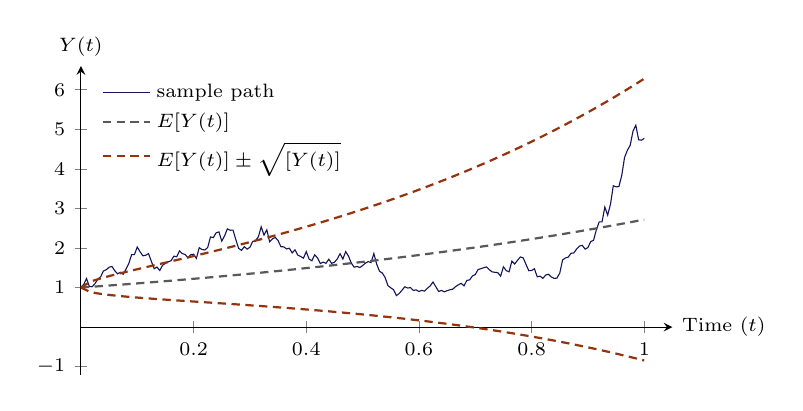
\begin{tikzpicture}[font=\footnotesize]
		\begin{axis}[
				width=0.75\textwidth, height=5.5cm,
				xmin=0, xmax=1.05, ymin=-1.2, ymax=6.6,
				xlabel={Time ($t$)}, ylabel={$Y(t)$},
				axis lines=middle, axis line style={thin},
				xlabel style={at={(ticklabel* cs:1)}, anchor=west},
				ylabel style={at={(ticklabel* cs:1)}, anchor=south},
				label style={font=\scriptsize}, tick label style={font=\scriptsize},
				xtick={0.2,0.4,0.6,0.8,1}, ytick={-1,1,2,3,4,5,6},
				legend style={font=\scriptsize, draw=none, fill=none, at={(0.02,0.98)}, anchor=north west},
				legend cell align=left,
			]
			\addplot[MidnightBlue!80!black, thin] coordinates {(0.000,1.000) (0.005,1.080) (0.010,1.228) (0.015,1.027) (0.020,1.020) (0.025,1.099) (0.030,1.212) (0.035,1.272) (0.040,1.418) (0.045,1.451) (0.050,1.512) (0.055,1.535) (0.060,1.427) (0.065,1.347) (0.070,1.387) (0.075,1.335) (0.080,1.464) (0.085,1.608) (0.090,1.831) (0.095,1.832) (0.100,2.025) (0.105,1.905) (0.110,1.802) (0.115,1.817) (0.120,1.858) (0.125,1.664) (0.130,1.476) (0.135,1.517) (0.140,1.431) (0.145,1.563) (0.150,1.611) (0.155,1.650) (0.160,1.679) (0.165,1.793) (0.170,1.778) (0.175,1.925) (0.180,1.859) (0.185,1.835) (0.190,1.753) (0.195,1.833) (0.200,1.842) (0.205,1.738) (0.210,2.007) (0.215,1.961) (0.220,1.950) (0.225,2.010) (0.230,2.280) (0.235,2.262) (0.240,2.383) (0.245,2.406) (0.250,2.175) (0.255,2.306) (0.260,2.484) (0.265,2.449) (0.270,2.452) (0.275,2.211) (0.280,1.990) (0.285,1.940) (0.290,2.033) (0.295,1.972) (0.300,2.018) (0.305,2.166) (0.310,2.186) (0.315,2.283) (0.320,2.535) (0.325,2.327) (0.330,2.459) (0.335,2.158) (0.340,2.230) (0.345,2.268) (0.350,2.188) (0.355,2.033) (0.360,2.029) (0.365,1.976) (0.370,1.994) (0.375,1.875) (0.380,1.954) (0.385,1.820) (0.390,1.786) (0.395,1.742) (0.400,1.910) (0.405,1.722) (0.410,1.677) (0.415,1.828) (0.420,1.749) (0.425,1.606) (0.430,1.643) (0.435,1.613) (0.440,1.716) (0.445,1.612) (0.450,1.638) (0.455,1.721) (0.460,1.856) (0.465,1.721) (0.470,1.908) (0.475,1.795) (0.480,1.617) (0.485,1.515) (0.490,1.535) (0.495,1.505) (0.500,1.556) (0.505,1.616) (0.510,1.657) (0.515,1.631) (0.520,1.859) (0.525,1.593) (0.530,1.413) (0.535,1.367) (0.540,1.254) (0.545,1.049) (0.550,0.994) (0.555,0.945) (0.560,0.797) (0.565,0.849) (0.570,0.933) (0.575,1.021) (0.580,0.987) (0.585,1.000) (0.590,0.926) (0.595,0.942) (0.600,0.900) (0.605,0.929) (0.610,0.909) (0.615,0.981) (0.620,1.042) (0.625,1.140) (0.630,1.021) (0.635,0.900) (0.640,0.928) (0.645,0.893) (0.650,0.921) (0.655,0.943) (0.660,0.958) (0.665,1.024) (0.670,1.068) (0.675,1.107) (0.680,1.042) (0.685,1.180) (0.690,1.194) (0.695,1.294) (0.700,1.328) (0.705,1.456) (0.710,1.476) (0.715,1.502) (0.720,1.521) (0.725,1.450) (0.730,1.396) (0.735,1.385) (0.740,1.377) (0.745,1.288) (0.750,1.525) (0.755,1.427) (0.760,1.399) (0.765,1.668) (0.770,1.596) (0.775,1.689) (0.780,1.774) (0.785,1.752) (0.790,1.588) (0.795,1.426) (0.800,1.429) (0.805,1.476) (0.810,1.271) (0.815,1.288) (0.820,1.232) (0.825,1.316) (0.830,1.336) (0.835,1.266) (0.840,1.231) (0.845,1.239) (0.850,1.366) (0.855,1.699) (0.860,1.748) (0.865,1.769) (0.870,1.865) (0.875,1.876) (0.880,1.977) (0.885,2.049) (0.890,2.067) (0.895,1.971) (0.900,2.011) (0.905,2.163) (0.910,2.195) (0.915,2.465) (0.920,2.659) (0.925,2.659) (0.930,3.035) (0.935,2.830) (0.940,3.104) (0.945,3.574) (0.950,3.545) (0.955,3.554) (0.960,3.836) (0.965,4.288) (0.970,4.470) (0.975,4.595) (0.980,4.956) (0.985,5.103) (0.990,4.736) (0.995,4.725) (1.000,4.772)};
			\addlegendentry{sample path}
			\addplot[Gray!70!black, thick, densely dashed, domain=0:1, samples=60] {exp(x)};
			\addlegendentry{$E[Y(t)]$}
			\addplot[RawSienna, thick, densely dashed, domain=0:1, samples=60] {exp(x)+exp(x)*sqrt(exp(x)-1)};
			\addlegendentry{$E[Y(t)]\pm\sqrt{\Var[Y(t)]}$}
			\addplot[RawSienna, thick, densely dashed, domain=0:1, samples=60, forget plot] {exp(x)-exp(x)*sqrt(exp(x)-1)};
		\end{axis}
	\end{tikzpicture}
	\caption{A sample path of geometric Brownian motion with $\mu=0.5$, $\sigma=1$, so
		$E[Y(t)]=e^{t}$ and $\sqrt{\Var[Y(t)]}=e^{t}\sqrt{e^{t}-1}$. The lower band
		goes negative although $Y(t)>0$ always: one standard deviation is a poor
		description of a skewed distribution.}
	\label{fig:gbm}
\end{figure}

\zh{圖：$\mu=0.5$、$\sigma=1$ 的 geometric Brownian motion 樣本路徑，虛線是 $E[Y(t)]=e^{t}$ 和加減一個標準差。下方那條會變成負的，但 $Y(t)$ 永遠為正——對偏斜的分布，「平均 $\pm$ 一個標準差」描述得很差。}

\subsection{An Argument for Long-Term Investment}

\source{Slide p.~587}

Suppose the stock follows the geometric Brownian motion\footnote{Contributed by Dr.~King, Gow-Hsing on April 9, 2015. See \url{http://www.cb.idv.tw/phpbb3/viewtopic.php?f=7&t=1025}.}
\[
	S(t) \;=\; S(0)\,e^{N(\mu t,\sigma^{2}t)} \;=\; S(0)\,e^{tN(\mu,\sigma^{2}/t)} , \qquad t\ge0 ,
\]
where $\mu>0$.
The annual rate of return has a normal distribution:
\[
	N\left(\mu,\ \frac{\sigma^{2}}{t}\right) .
\]
The larger the $t$, the likelier the return is positive.
The smaller the $t$, the likelier the return is negative.

\zh{設股價服從 geometric Brownian motion $S(t)=S(0)e^{N(\mu t,\sigma^{2}t)}$，$\mu>0$。年化報酬率 $\sim N(\mu,\sigma^{2}/t)$：持有越久，報酬為正的機率越高；越短則越可能是負的。}

\begin{remark}
	\begin{enumerate}[(1),nosep]
		\item \textbf{$e^{N(\mu t,\sigma^{2}t)}=e^{tN(\mu,\sigma^{2}/t)}$。}若 $Z\sim N(\mu,\sigma^{2}/t)$，則 $tZ\sim N(\mu t,t^{2}\cdot\sigma^{2}/t)=N(\mu t,\sigma^{2}t)$。
		\item \textbf{年化報酬率。}連續複利的年化報酬率 $\frac1t\ln\frac{S(t)}{S(0)}=Z\sim N(\mu,\sigma^{2}/t)$。
		\item \textbf{報酬為正的機率。}$\mathrm{Prob}[Z>0]=N\bigl(\mu/\sqrt{\sigma^{2}/t}\bigr)=N\bigl(\mu\sqrt{t}/\sigma\bigr)$，$\mu>0$ 時隨 $t$ 遞增、$t\to\infty$ 時趨近 $1$；$t\to0$ 時趨近 $N(0)=1/2$。
	\end{enumerate}
\end{remark}

\begin{note}
	這個論證說的是\emph{年化}報酬率的不確定性 $\sigma/\sqrt{t}$ 會縮小；總 log 報酬 $\ln(S(t)/S(0))$ 的標準差 $\sigma\sqrt{t}$ 仍然隨 $t$ 增加。所以長期持有讓「虧錢」的機率變小，但不代表財富的絕對波動變小。
\end{note}
